\documentclass[11pt,a4paper]{article}

\usepackage{mynotes}

\graphicspath{ {img/} }  % Define image path

\renewcommand{\lstlistingname}{Code}

\addbibresource{workflow.bib}

\usepackage{placeins}

% Variables
\newcommand{\mispreps}{20}
\newcommand{\minreps}{100}
\newcommand{\minsp}{9}
\newcommand{\wireps}{20}
\newcommand{\wikn}{50}
\newcommand{\wiki}{100}

\newcommand{\hemiCor}{$r$(195) = 0.89, p<0.001}


\title{Estimation of woodland canopy structure with terrestrial LiDAR: expanded methods}
\author{John L. Godlee}
\date{\today}

% Body
\begin{document}

\maketitle{}

\linenumbers

\section{Introduction}

This chapter provides expanded field and analytical methods for the study of tree canopy structure in southern African woodlands, presented in brief in Chapter 5. The study aimed to understand the effects of tree species diversity and stand structure on tree canopy structural complexity, using terrestrial LiDAR. Firstly, I provide technical details on the field setup for the terrestrial LiDAR and the hemispherical photography used to validate terrestrial LiDAR canopy closure estimates. Secondly, I describe the processing chain used to extract canopy complexity metrics from the terrestrial LiDAR point clouds. Thirdly, I describe in further detail the behaviour and suitability of the different canopy complexity metrics and stand structural metrics used in the study.

\section{Terrestrial LIDAR field setup}

Within each 1 ha (100x100 m) square plot, nine 10 m diameter circular subplots were laid out in a grid, with 35 m between subplot centre points (\autoref{subplot_plot}). These subplots constitute the basic sampling unit of the study. Within each subplot, a Leica HDS6100 phase-shift Terrestrial Laser Scanner (TLS) was used to capture woodland canopy structure. The number and position of scan locations within a subplot was determined by the arrangement and density of canopy material in the subplot. Scan positions were arranged to minimise shadows within the canopy, and to maximise canopy penetration. Between one and five scans were recorded per subplot, across all plots. Further information on the field setup of the TLS is presented in \autoref{scan_settings}.

Five Leica 6" (15.24 cm) diameter planar tilt-and-turn cross-pattern reflective targets were used in each subplot to align scans (\autoref{target}). The five targets were located roughly in a quincunx pattern, with one target at the subplot centre and the remaining four targets arranged in a cross pattern around the edges of the subplot, ensuring that all scans could see all five targets. To facilitate alignment of scans among subplots, the location of each target in real space was recorded using a Leica VIVA GS10 GNSS (Global Navgation Satellite Systems) unit (\autoref{viva}). The GNSS was set up in a Post-Processing Kinematic (PPK) configuration with a base-station located \textasciitilde{}100 m from the edge of each 1 ha plot with an unobstructed view of the sky hemisphere where possible. The location of each target was measured for at least 4 minutes to minimise measurement error (\autoref{ppk}). 

\begin{figure}
	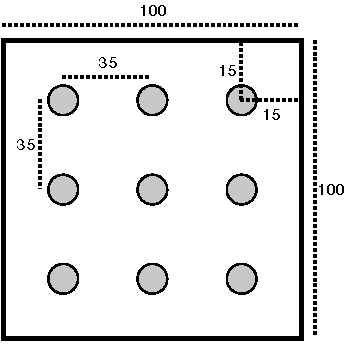
\includegraphics[width=0.5\linewidth]{plot}
	\caption{The layout of 10 m diameter subplots within each 1 ha plot. Each subplot is situated inside a 15 m buffer from the plot edge, with 35 m between subplot centres. Subplots are arranged in a 3x3 grid. All distances are in metres.}
	\label{subplot_plot}
\end{figure}

\begin{figure}
	\begin{subfigure}{0.45\linewidth}
		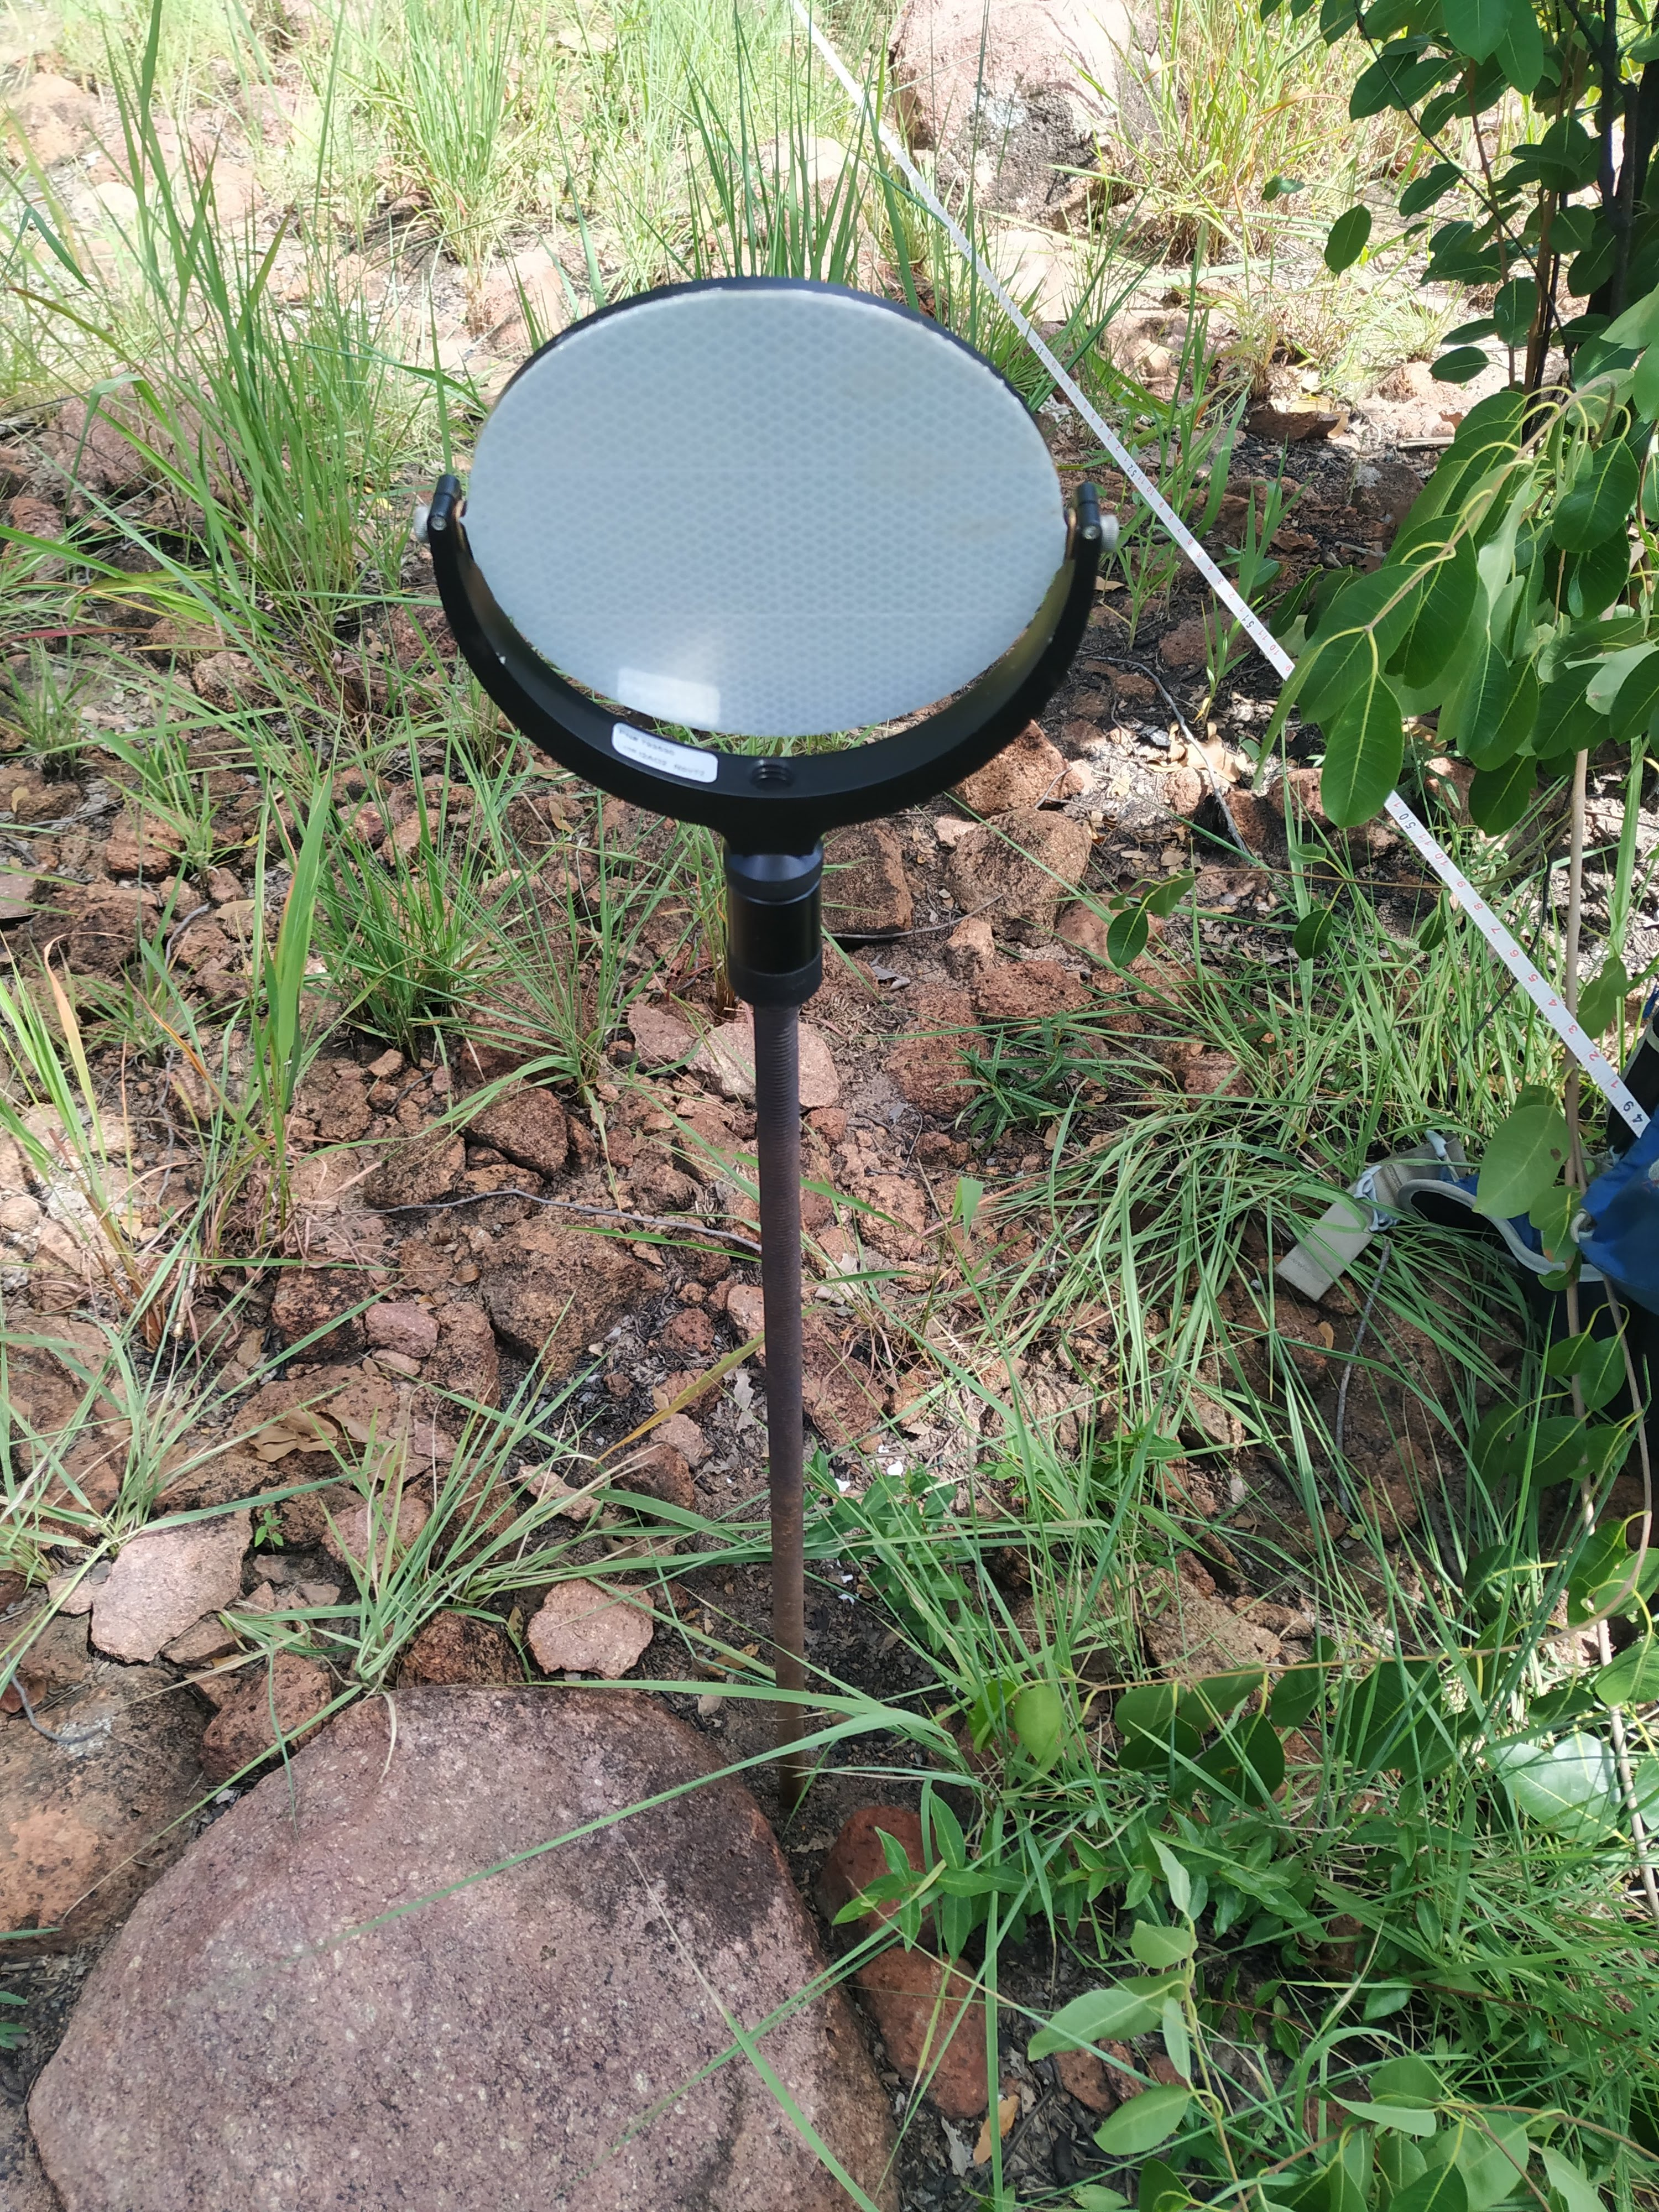
\includegraphics[width=\linewidth]{target_situ}
		\caption{}
		\label{target_situ}
	\end{subfigure}
	\hfill
	\begin{subfigure}{0.45\linewidth}
		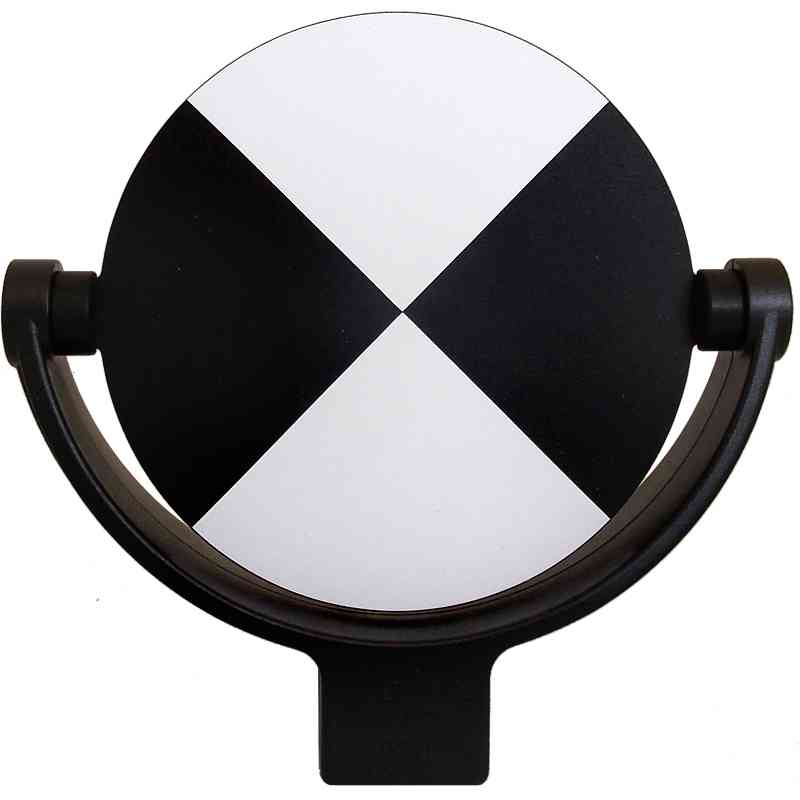
\includegraphics[width=\linewidth]{target_face}
		\caption{}
		\label{target_face}
	\end{subfigure}
	\caption{Example of a Leica 6" diameter reflective target, (a) in situ mounted on a length of threaded bar, and (b) showing the cross pattern face of the target.}
	\label{target}
\end{figure}

\begin{figure}
	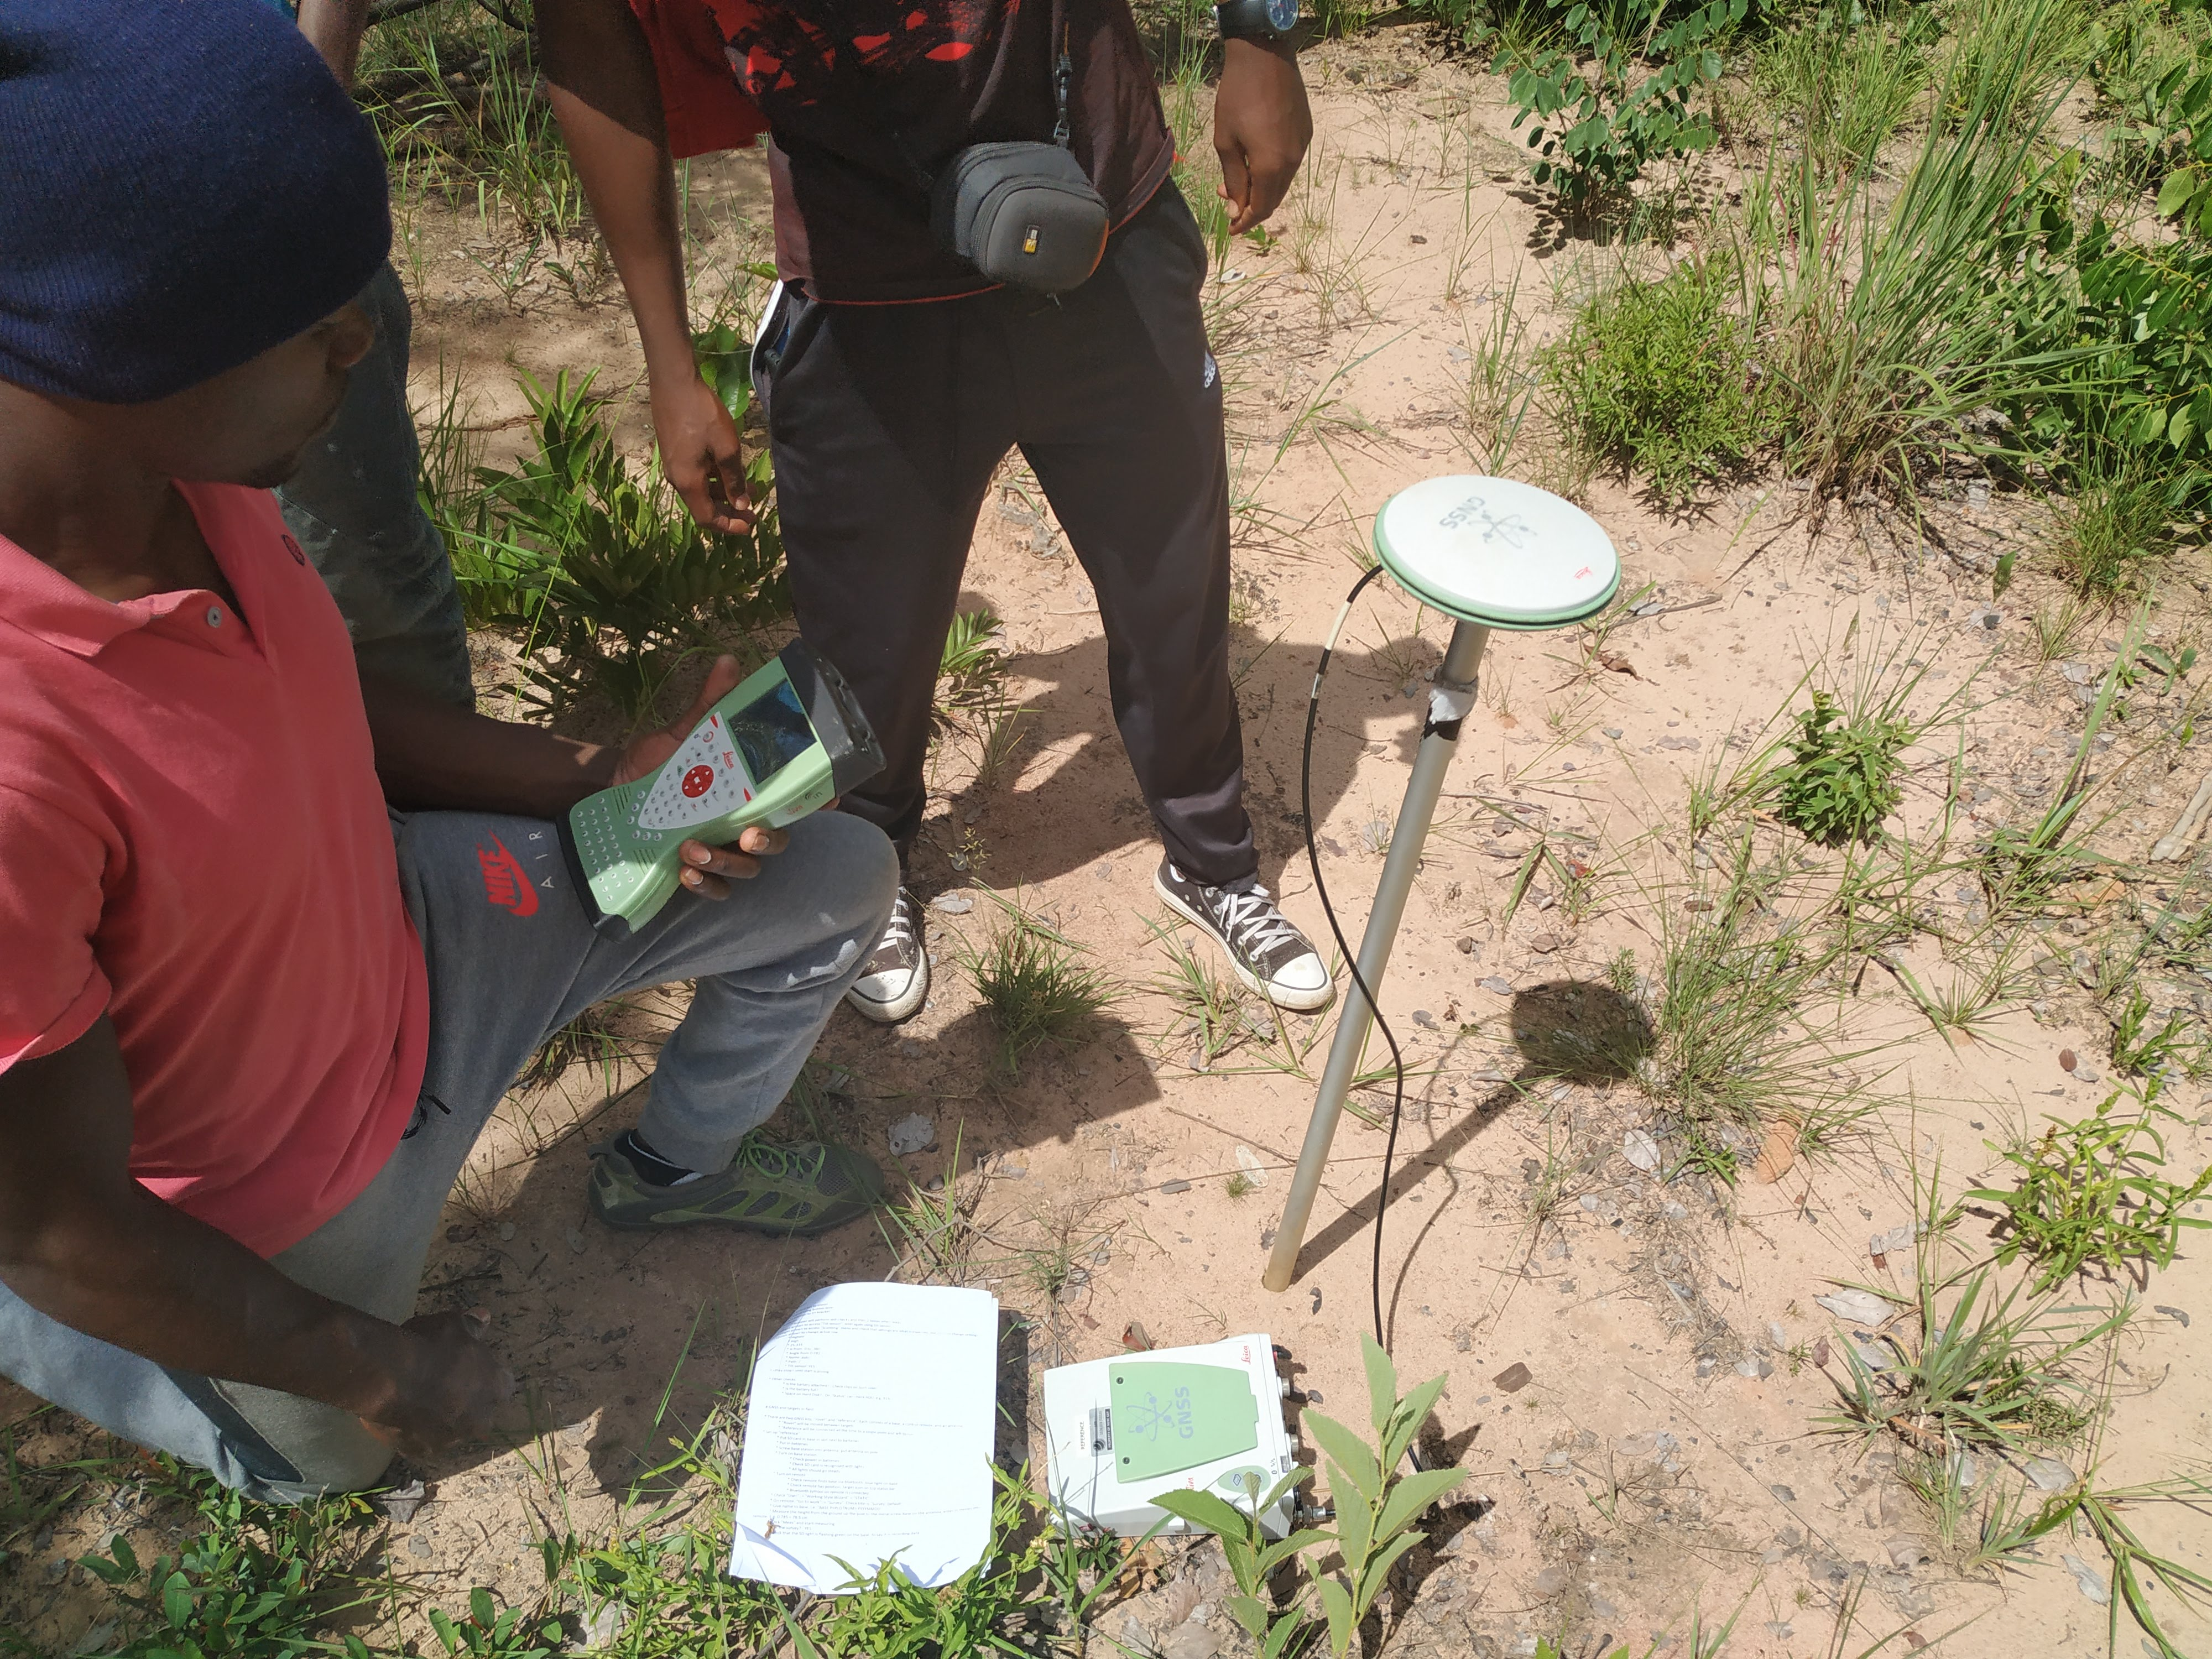
\includegraphics[width=0.6\linewidth]{viva}
	\caption{A Leica VIVA GS10 GNSS unit in the field, showing the antenna atop an aluminium pole, attached to the base station on the ground, and the rover terminal in the hand of a research assistant.}
	\label{viva}
\end{figure}

\begin{figure}
	\frame{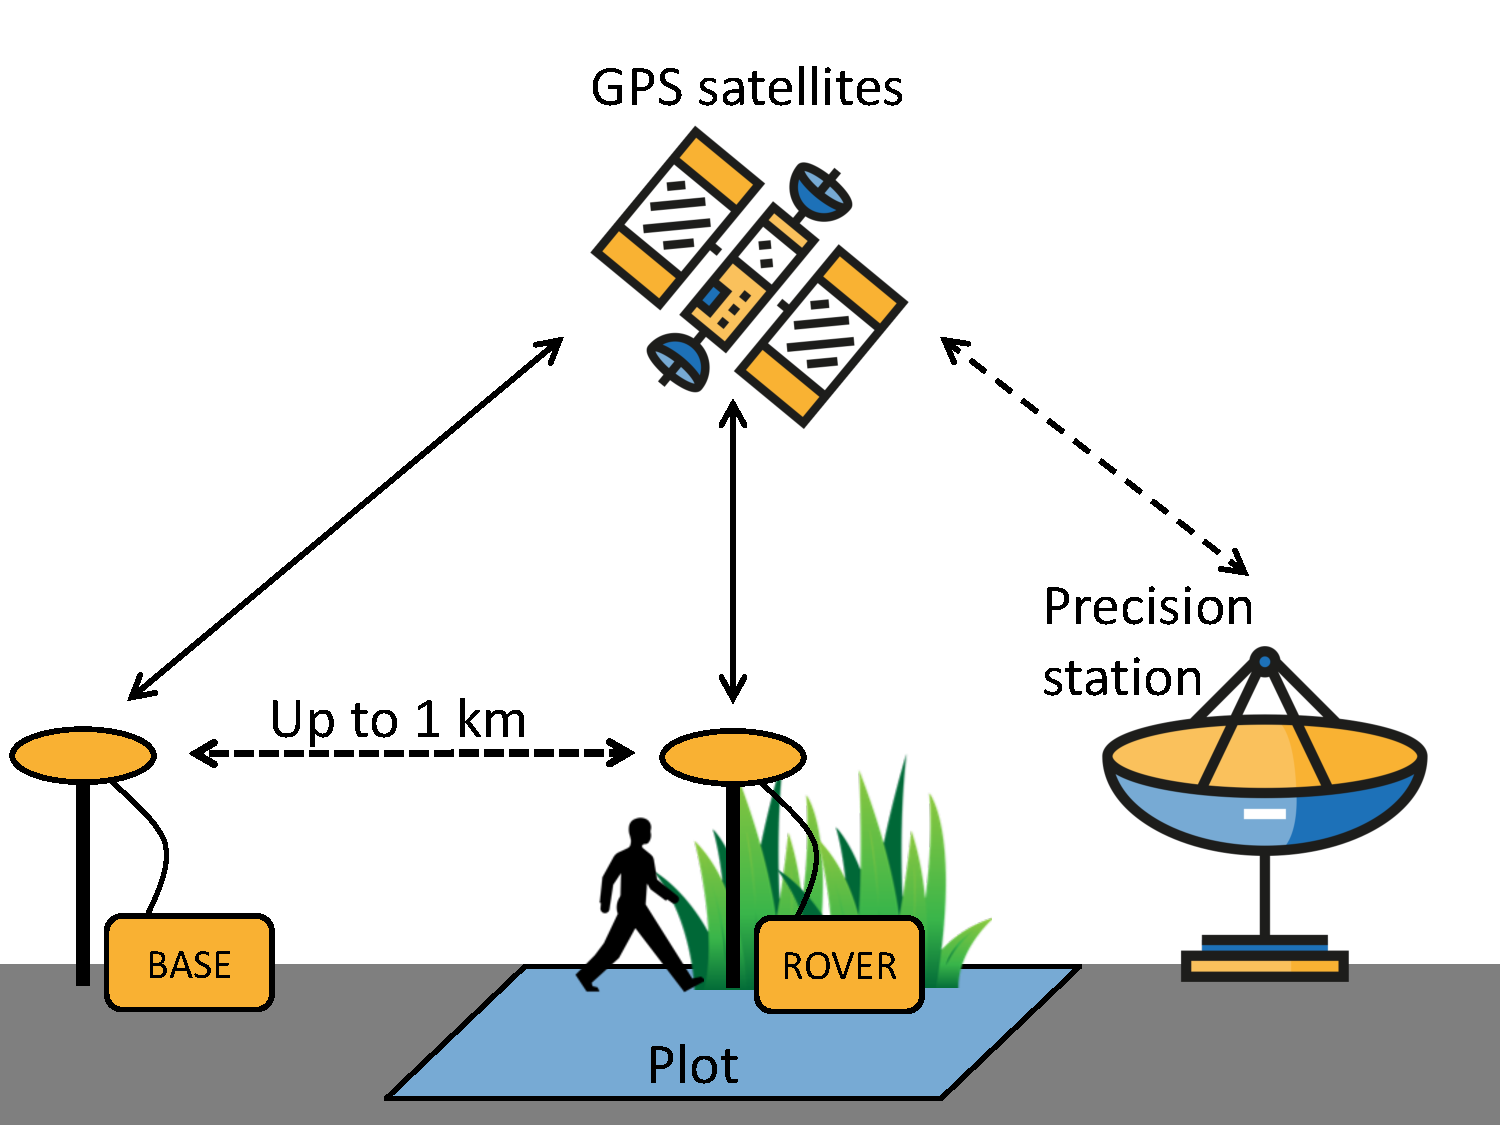
\includegraphics[width=0.8\linewidth]{ppk}}
	\caption{Schematic diagram of the GNSS PPK configuration used to precisely locate targets in real space. The base station is located in an area with a full unobstructed view of the sky hemisphere, up to \textasciitilde{}1 km from the plot, and is left in the same location for the duration of the data collection, recording its location once per second. The rover is moved around inside the plot to record the location of each target, for >4 minutes at each target. The rover and the base station both utilise GPS and GLONASS satellites to record their position. After data collection, a two stage validation technique is used to improve the precision of the recorded positions, firstly using the base station, and secondly using the TrimbleRTX service which utilises highly precise distributed regional stations.}
	\label{ppk}
\end{figure}

\begin{table} \centering 
  \caption{Description of scan settings used for each scan.} 
  \label{scan_settings} 
\begin{tabular}{@{\extracolsep{0pt}} rl} 
\\[-1.8ex]\hline 
\hline \\[-1.8ex] 
{Setting} & {Value} \\
\hline \\[-1.8ex] 
TLS model & Leica HDS6100 \\
Wavelength & 650-690 nm \\
Spot size at exit & 3 mm \\
Beam divergence & 0.22 mrad \\
Range & 79 m @90\%; 50 m @18\% albedo \\
Azimuth range & 0-360\textdegree{} \\
Zenith range & 0-155\textdegree{} \\
Increment & 0.018\textdegree{} \\
Point spacing over 25 m & 7.9 mm \\
Pixels per line & \num{20000} \\
Lines & \num{10000} \\
Compressed file size & \textasciitilde{}800 MB \\
Duration of scan & 6 minutes 44 seconds \\
\hline
\hline \\[-1.8ex] 
\end{tabular} 
\end{table} 


\section{Hemispherical photography field setup}

In order to validate TLS canopy closure estimates, at the centre of each subplot a single photograph was taken with a full-frame DSLR camera, equipped with a circular fisheye lens. Further information on the hemispherical photography setup is presented in \autoref{camera_settings}.

The fisheye lens had an equisolid (equal area) projection, with a projection function given by: 

\begin{equation}
	R = 2f \sin{(\frac{\theta{}}{2})}
\end{equation}

Where $R$ is the radial position of a point on the image, $f$ is the focal length of the lens, and $\theta{}$ is the angle in radians of incident light on the lens. Equisolid lenses are preferred for hemispherical photography because they maintain an equal area for each pixel, i.e. a pixel projected through the lens has the same solid angle irrespective of the incident light angle, meaning that canopy closure estimations are not biased towards any part of the sky hemisphere \citep{Herbert1987}.

Photographs were taken facing directly to zenith using a camera-mounted spirit level, with the top of the camera body facing magnetic north, at a height of 1.3 m or above understorey vegetation, whichever was higher. Photographs were captured under uniform light conditions as much as possible, either under overcast skies or early in the day before direct sunlight could be seen on the photograph, to minimise lens flare, which can preclude accurate differentiation of plant material and sky, and `blooming', a phenomenon where light `bleeds' into dark areas of the image in highly contrasting light conditions \citep{Frazer2001}.

ImageJ (Fiji version 2.1.0/1.53c) was used to binarise hemispherical photographs, to separate plant material from sky \citep{Schneider2012}. Images were binarised using the Huang algorithm \citep{Huang1995} using only the blue channel of the image, under the assumption that plant material reflects little blue light, while the sky reflects much more \citep{Brusa2014}. Images were saved as PNG files at the original pixel resolution, with a circular image of 4016x4016 pixels.

\begin{table}
\centering 
  \caption{Description of camera settings used for hemispherical photographs. Note that shutter speed and ISO are deliberately variable within sensible thresholds to allow adjustments for ambient light conditions.} 
  \label{camera_settings} 
\begin{tabular}{rl} 
	\toprule
{Setting} & {Value} \\
	\midrule
Camera model & Nikon D750 \\
Lens model & Sigma 8 mm f/3.5 EX DG Circular Fisheye \\
Pixel pitch & \SI{5.95}{\micro\meter} \\
Sensor resolution & 24.3 MP \\
Shutter speed & >1/60s \\
Aperture & 5-7 \\
ISO & 100-200 \\
Exposure compensation & -0.7 \citep{Brusa2014} \\
Focus & $\infty$ \citep{Hu2009, Frazer2001}\\
Image size & Large Fine JPEG - circular image 4016x4016 px \\
Orientation & Landscape \\
\bottomrule
\end{tabular} 
\end{table} 

\section{Terrestrial LiDAR processing}


\begin{figure}
\centering
	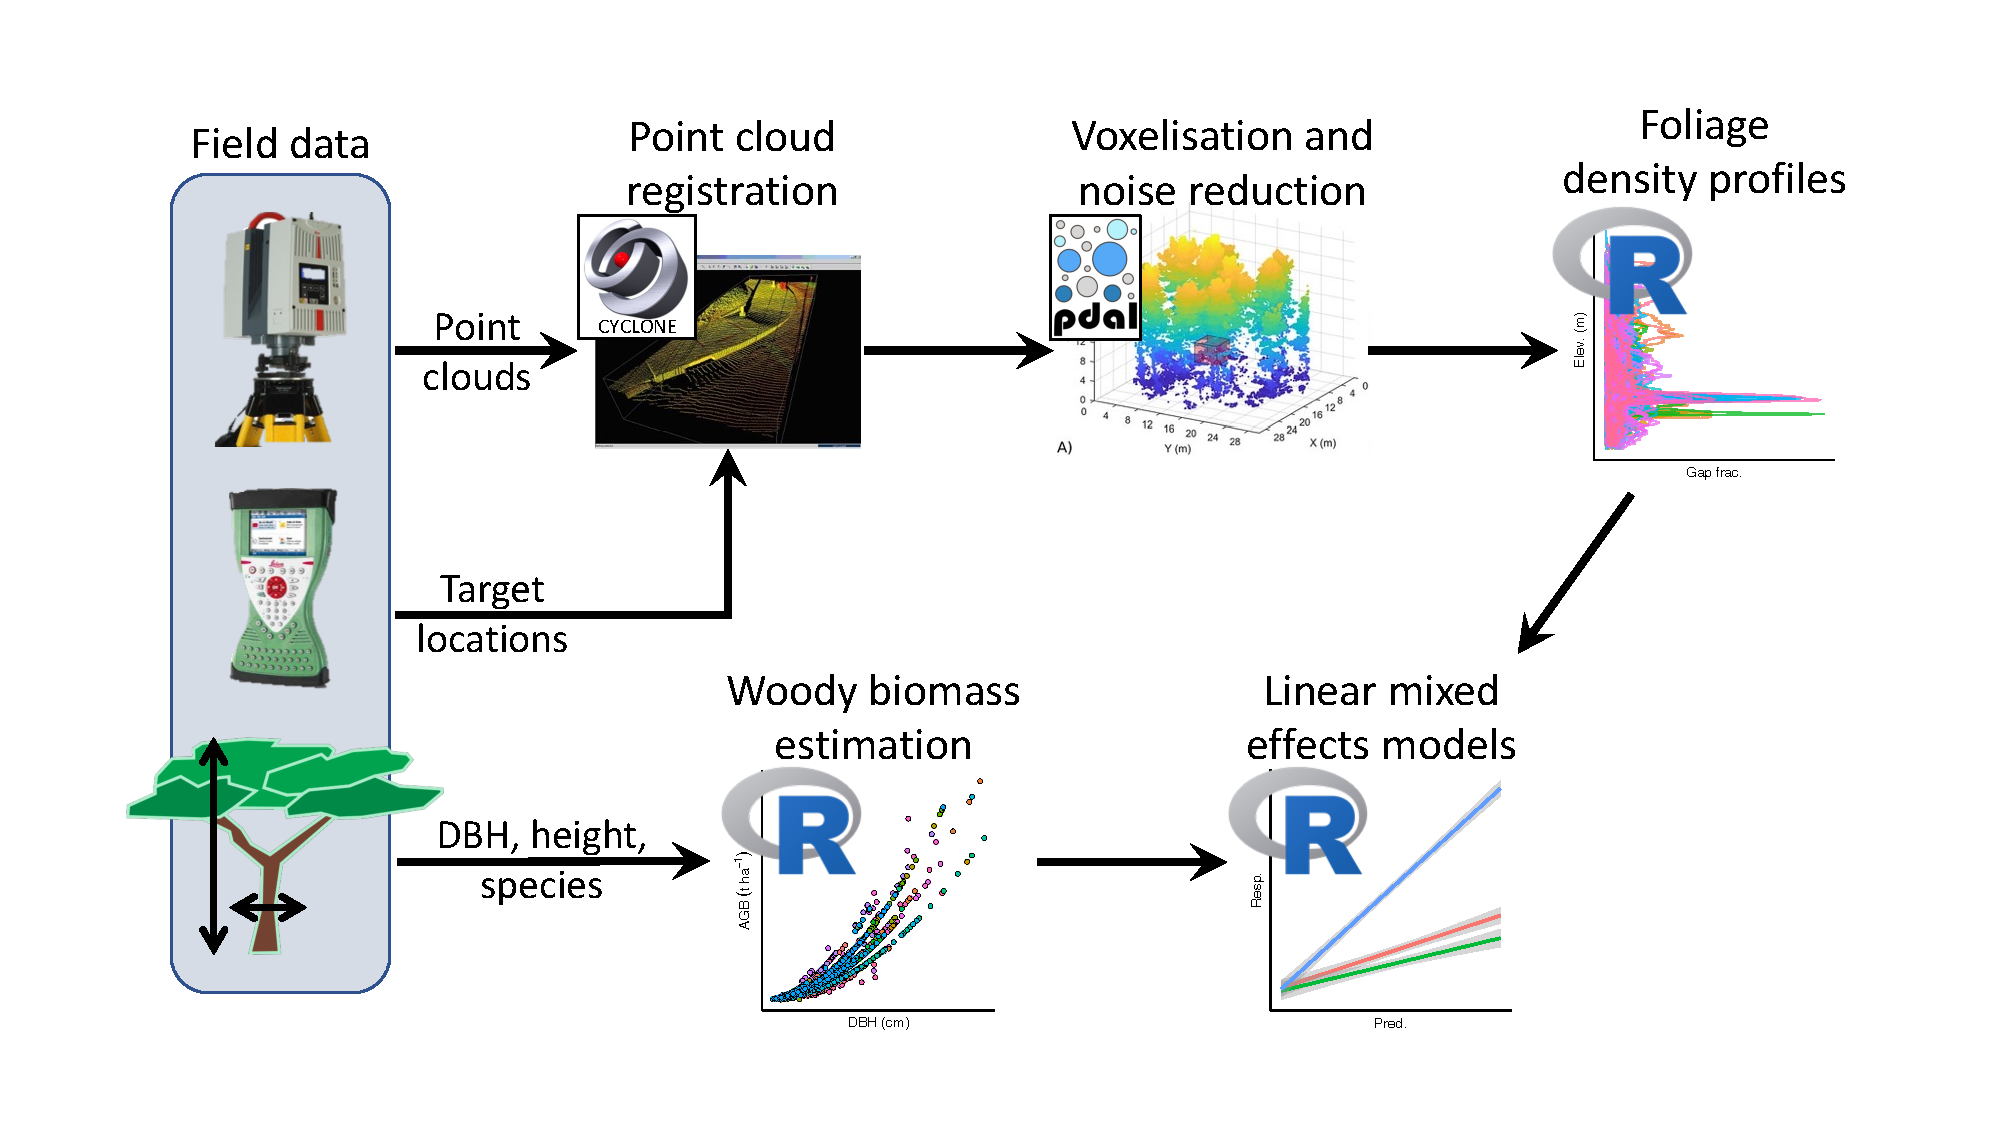
\includegraphics[width=\linewidth]{workflow_diag}
	\caption{Schematic diagram summarising the data processing and analysis workflow for the TLS data. Processing steps are labelled according to the principal software used during that step.}
	\label{workflow_diag}
\end{figure}

\subsection{Scan alignment and registration}

Point clouds within a subplot were aligned using the reflective targets as anchor points. Point cloud alignment was conducted in Leica Cyclone (version 9.1) \citep{Cyclone}. Reflective targets were manually located within each point cloud, then the precise centre of each target was identified automatically by Cyclone. Anchor points were discarded if they had a location uncertainty of >3 cm. After alignment, subplot point clouds were exported from Cyclone as PTX files for further processing.

GNSS target locations were used to register point clouds in real space. The TrimbleRTX GNSS post-processing service was used to improve the precision of target locations recorded with GNSS, using distributed regional stations to validate the rover and base station GNSS measurements (\autoref{auspos_close}) \citep{Chen2011}. Following point cloud registration, subplot point clouds were combined to a plot-level point cloud.

% latex table generated in R 4.1.0 by xtable 1.8-4 package
% Sat Aug 21 08:22:54 2021
\begin{table}[]
\centering
\caption{The five closes regional base stations to each site, used by TrimbleRTX to refine GNSS measurements} 
\label{auspos_close}
\begin{tabular}{llS[table-format=4.0]}
  \toprule
{Site} & {Receiver} & {Distance (km)} \\ 
  \midrule
{\multirow{5}{*}{Bicuar}} & JAVAD TRE 3 & 863 \\ 
   & JAVAD TRE 3 DELTA & 1448 \\ 
   & TRIMBLE NETRS & 1630 \\ 
   & TRIMBLE NETRS & 1648 \\ 
   & JAVAD TRE G3TH DELTA & 1796 \\ 
   \midrule
{\multirow{5}{*}{Mtarure}} & SEPT POLARX5 & 686 \\ 
   & TRIMBLE ALLOY & 795 \\ 
   & LEICA GRX1200GGPRO & 903 \\ 
   & JAVAD TRE 3 DELTA & 1119 \\ 
   & JAVAD TRE 3 DELTA & 1315 \\ 
   \bottomrule
\end{tabular}
\end{table}



PTX files were converted to compressed LAZ files using PDAL \citep{PDAL}, to reduce file size and speed up further processing. \autoref{ptx_laz} contains the code used to transform PTX to LAZ. 

\vspace{\baselineskip}
\begin{minipage}{\linewidth}
\lstinputlisting[label=ptx_laz,language=bash,caption={The processing chain used to convert Leica Cyclone PTX files to LAZ files, using PDAL, POSIX shell scripting, and common UNIX utilities. The \texttt{ptx\_laz.json} JSON pipeline is shown in \autoref{ptx_laz_json}.}]{inc/ptx_laz.txt}
\end{minipage}

\vspace{\baselineskip}
\begin{minipage}{\linewidth}
	\lstinputlisting[label=ptx_laz_json,language=json,caption={The JSON pipeline used in \autoref{ptx_laz} to convert PTX files to LAZ files, and applying a rotation matrix.}]{inc/ptx_laz_json.txt}
\end{minipage}

\subsection{Voxelisation}

Point clouds were voxelised to different voxel sizes depending on the application of the data. 5 cm\textsuperscript{3} cubic voxels were used for subplot height profile estimation, while 50 cm\textsuperscript{3} voxels were used for whole plot canopy rugosity. Variation in voxel size reflects the spatial scale of each analysis, and is bounded by the beam divergence of the scanner over longer distances \citep{Grau2017}. Choosing voxels that are too small can result in pock-marked representations of surfaces that are especially problematic when calculating larger scale canopy structure metrics such as canopy top roughness, while voxels that are too large can result in an over-estimation of plant volume when estimating canopy foliage density at the subplot scale, especially when foliage is clumped \citep{Seidel2012, Cifuentes2014}. Voxels were classified as `filled' if they intersected one or more points. 

\subsection{Noise reduction}

Outlier detection and noise reduction of point clouds was conducted in PDAL, using the ``statistical method'' (sensu \citealt{Rusu2008}) of \texttt{filters.outlier}, with $k = 8$ (mean number of neighbours), and $m = 1.96$ (outlier distance threshold multiplier, here approximating a 95\% confidence interval):

\begin{align}
\begin{split}
	\overline{\mu} &= \frac{1}{N} \sum_{i=1}^{N} \mu_{i} \\
	\sigma &= \sqrt{\frac{1}{N-1} \sum_{i=1}^{N}(\mu_{i} - \overline{\mu{}})^2} \\
	t &= \mu + m \sigma \\
	\text{with}\ outlier_{i} &= 
		\begin{cases}
			\text{true},& \text{if}\ \mu_{i} >= t \\
			\text{false},& \text{otherwise}
		\end{cases}
\end{split}
\end{align}

Where $\mu_{i}$ is the mean distance from point $i$ to all $k$ nearest neighbour points, $N$ is the number of points in the scene, $\overline{\mu}$ is the mean distance to nearest neighbour points, $\sigma$ is the standard deviation of these mean distances, $t$ is the threshold distance used to define an outlier and $outlier_{i}$ is the condition of a point in the scene being identified as an outlier.

\begin{figure}
\centering
	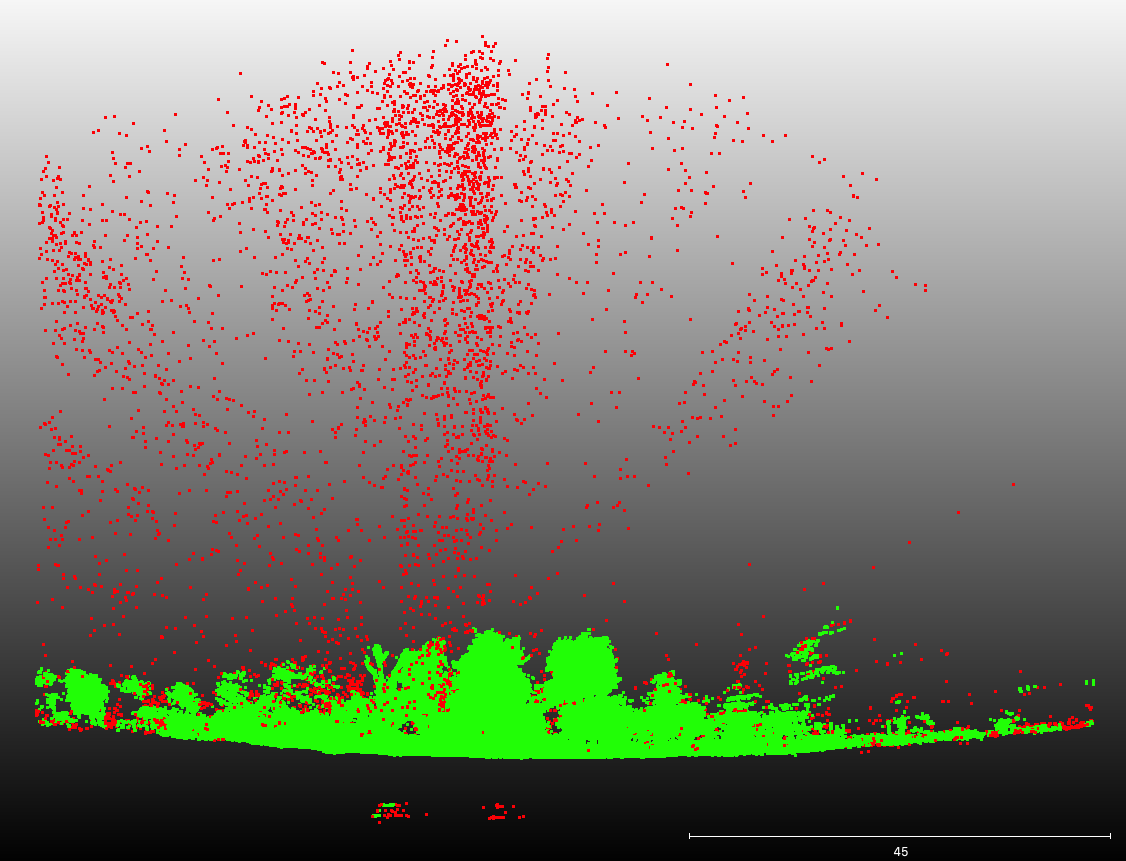
\includegraphics[width=\linewidth]{noise_vis}
	\caption{A 2 m deep cross section of a subplot point cloud showing the efficacy of the noise reduction and voxelisation process. Red points are excluded by the process, while green points are preserved for further analysis.}
	\label{noise_vis}
\end{figure}

\subsection{Foliage density profiles}

To calculate subplot foliage density profiles, the 5 cm\textsuperscript{3} voxelised point cloud was first cropped to a 10 m diameter cylinder of infinite height. Ground points were identified using \texttt{filters.pmf} (Progressive Morphological Filter - PMF) in PDAL (sensu \citealt{Zhang2003}), and the height above ground of all points was calculated using \texttt{filters.hag\_nn} (Nearest Neighbour) in PDAL. Points below ground level and above the 99.9th percentile of height were excluded from further analyses. Height profile points were exported to XYZ coordinates then imported into R for further processing. 

In R, foliage density was calculated in 5 cm layers as the proportion of filled 5 cm\textsuperscript{3} voxels. A loess model with a span of 0.1 was fitted to the foliage density values in each layer to estimate the foliage density profile (\autoref{height_profile_illus}). The foliage density profile was further filtered to only tree canopy material, by discarding all points below the first local minimum in the foliage density profile above 1.3 m, using a rolling window of 50 cm.

Multiple statistics were extracted from the foliage density profile for use in statistical analyses. Total canopy foliage density was calculated as the area under the curve of the canopy foliage density profile, using trapezoid estimation. The Effective Number of Layers (ENL) in the foliage density profile was used to estimate canopy structural complexity, using the true-numbers equivalent of the Shannon diversity index on the foliage density of 50 cm layers (sensu \citealt{Ehbrecht2016}):

\begin{equation}
	\text{ENL} = \text{exp}\Big{(} - \sum_{i=1}^{N} p_{i} \text{ln} p_{i} \Big{)}
\end{equation}

Where $N$ is the number of 50 cm bins in the height profile, and $p_{i}$ is the proportion of filled voxels in layer $i$ (foliage density). While \citet{Ehbrecht2016} used 1 m layers, their study was conducted in temperate deciduous forest where the maximum height of the sampled forest stands was 40 m, whereas the maximum canopy height in this study was only 22 m. Both \citet{Ehbrecht2016} and \citet{Montes2004} assert that layer thickness is largely arbitrary, but should be determined with respect to the variability within the canopy, thus in the sparse and highly variable savanna tree canopies measured in this study, narrower layers were chosen. 

To describe the uniformity of the foliage density distribution through the canopy, a linear model of foliage density with height was fitted. Under a completely even distribution of foliage material through the canopy, the residuals of the linear model tend to zero, while clumping causes deviations from this uniform distribution and increases the sum of residuals.

While maximum canopy height has been used in other studies to describe canopy structural complexity \citep{Scheuermann2018}. At the small spatial scale of the subplots used in this study however, there proved to be too much stochastic variation in canopy height among subplots due to the distribution of individual trees to make this statistic informative as a measure of canopy complexity. Canopy height was calculated later at the plot level, however. Similarly, previous studies have used the number of local maxima in the foliage density profile to estimate canopy structural complexity \citep{Wilkes2016}. However, this metric covaries with ENL and total foliage density, while ENL is uncorrelated with foliage density \citep{Ehbrecht2016}. 

\begin{figure}
\centering
	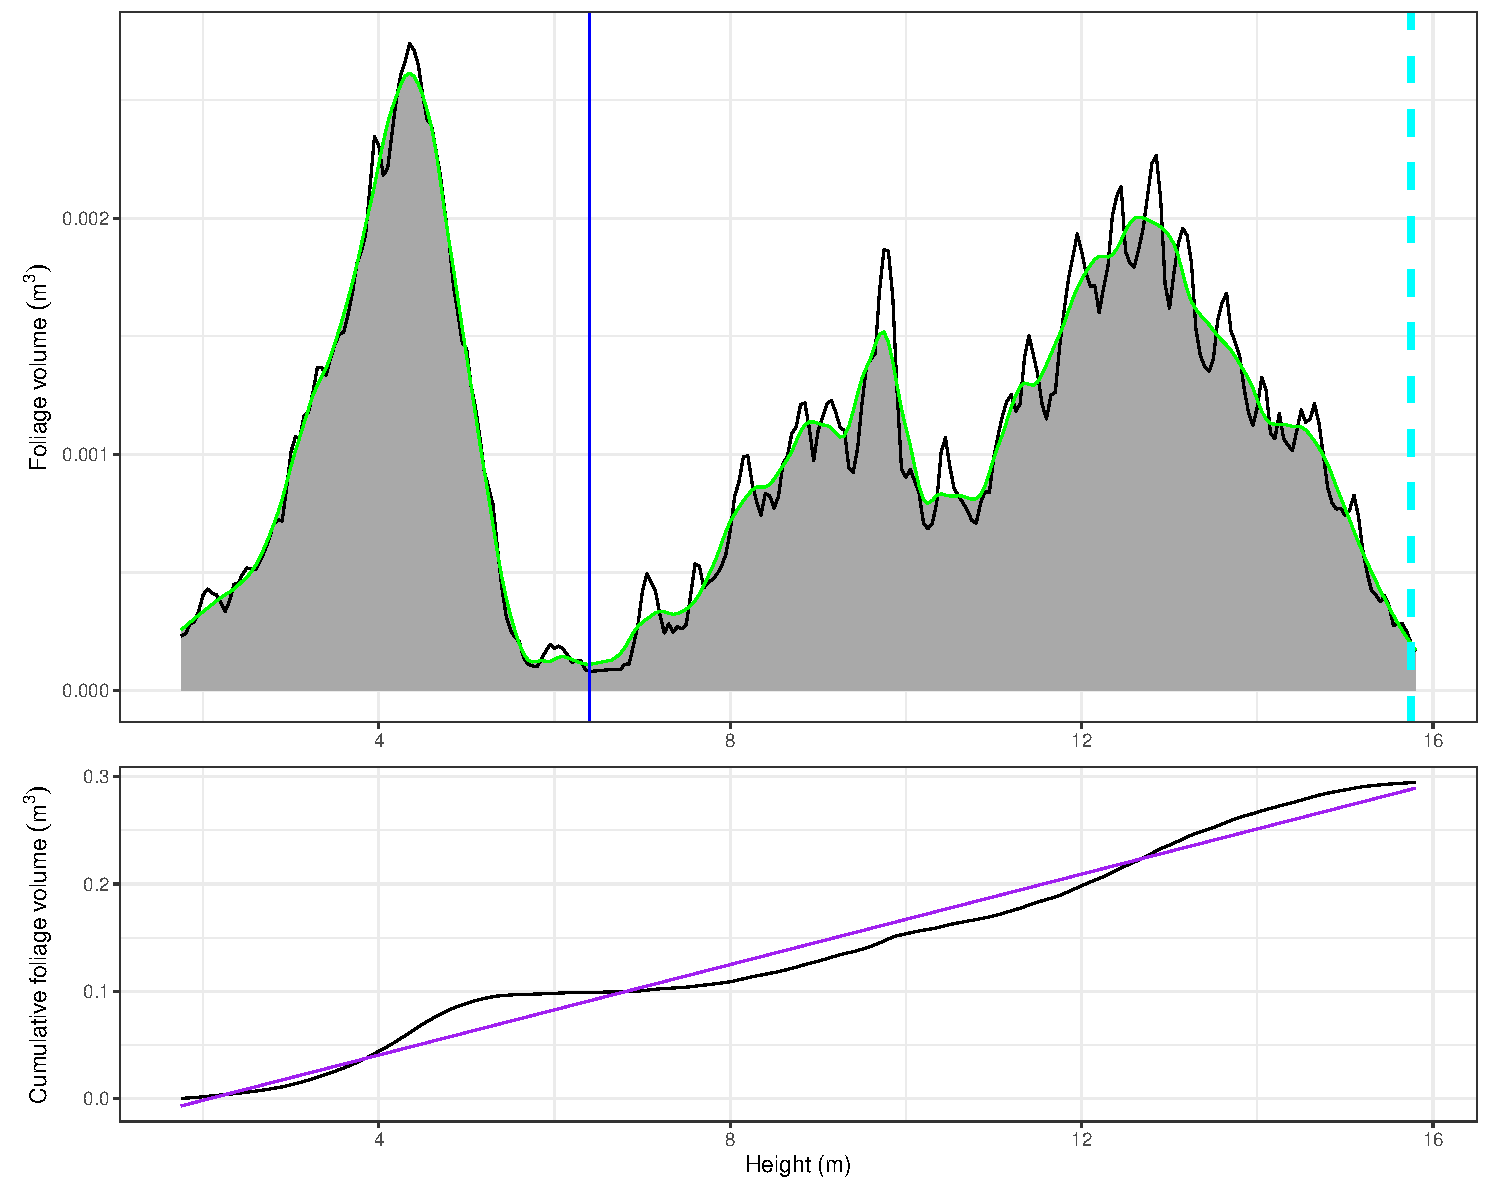
\includegraphics[width=\linewidth]{height_profile_illus_all}
	\caption{Subplot foliage volume height profile (top) and cumulative foliage volume profile (bottom) for a subplot in Bicuar National Park, Angola, to illustrate some of the canopy structure metrics extracted from each height profile. Starting with the top panel: the blue solid line represents the first local minimum above 1.3 m, used to define the base of the tree canopy. The dashed cyan line shows the 99.9th percentile of canopy height, used here as a measure of canopy top height across the subplot and in plot-level canopy surface modelling. The black trace shows the foliage density height profile, and the green trace shows the loess model fitted to the data, with the area under the canopy shaded grey. The bottom panel: the black trace shows the cumulative foliage volume through the canopy, taken from the loess fit in the top panel. The purple line shows the line of best fit of a linear model through this data. Not illustrated is the Effective Number of Layers (ENL) metric.}
	\label{height_profile_illus}
\end{figure}

\subsection{Canopy closure}

Subplot canopy closure, i.e. the proportion of the sky hemisphere occluded by plant material, a.k.a. gap fraction or site factor \citep{Jennings1999}, was measured by simulating a hemispherical image at the centre of the subplot using the point cloud data from all scans per subplot. The point cloud was first cropped to a 20 m diameter cylinder around the subplot centre using PDAL. Points below 1.3 m and within a 50 cm sphere around the subplot centre at 1.3 m height were discarded, to prevent the simulated hemispherical image being occluded by understorey vegetation. POV-Ray was used to simulate the hemispherical image using ray-tracing \citep{Povray2004}. Filled voxels were represented in POV-Ray as non-reflective black cubes filling the 5 cm\textsuperscript{3} voxel volume, with a white uniform sky box and no light source. POV-Ray produced an image with identical qualities to that of the real hemispherical photograph, using a fisheye lens with an equisolid projection and a view angle of 180\textdegree, located at the subplot centre at 1.3 m above the ground, with the top of the camera facing magnetic north and the camera facing directly to zenith, producing a circular image of 4016x4016 pixels.

Hemiphot \citep{HemiPhot} was used to estimate closure from both the hemispherical photographs and the TLS POV-Ray simulation. Hemiphot calculates canopy closure in 90 evenly sized concentric rings. To obtain the total closure of a circular image:

\begin{equation}
	C_{\alpha{}} = 1 - G_{\text{tot}} = \sum_{\alpha{} = 0.5}^{\alpha{} = 89.5}(G_{\alpha{}} A_{\alpha{}} / A_{\text{tot}})
\end{equation}

Where $G_{\alpha{}}$ is the fraction of unfilled pixels in ring $\alpha{}$, $A_{\alpha{}}$ is the sky area of the ring segment, and $A_{\text{tot}}$ is the total sky area of the hemisphere.

Canopy closure estimates from the TLS were validated using estimates from hemispherical photography. A Pearson's correlation analysis showed that both methods were highly correlated (\hemiCor{}). TLS estimates of closure were almost exclusively higher than hemispherical photography estimates, except in a few subplots with particularly low canopy closure. At higher canopy closure the over-estimation of canopy closure by TLS was larger (\autoref{tls_hemi_compare}). This finding is in agreement with previous studies which have found that that the magnitude of TLS canopy closure over-estimation depends on gap size distribution, where a site with greater canopy cover and a gap fraction dominated by small within crown gaps will have a larger over-estimate than a more open site with a gap fraction dominated by large between crown gaps \citep{Seidel2012}. A linear mixed model which accounted for the nested sampling of subplots within plots was used to identify if sites differed significantly in their relationship between hemispherical photography and TLS estimates of canopy closure. There was no significant difference in model fixed effect slope between plots in Bicuar National Park, Angola, and those in Mtarure, Tanzania (\hemiLme{}). 

\begin{figure}
\centering
	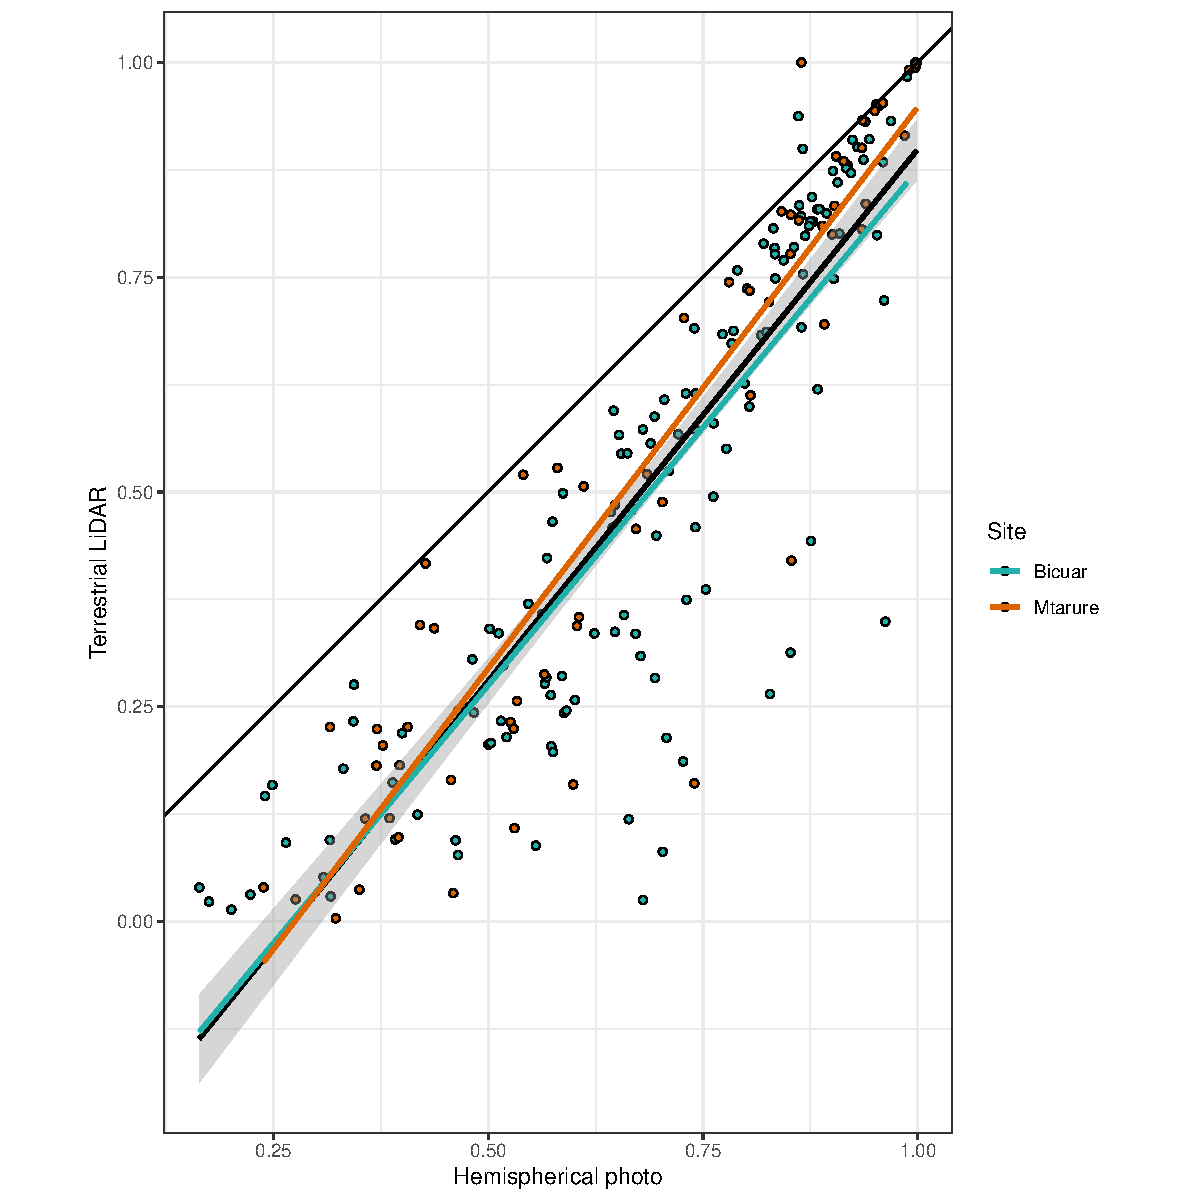
\includegraphics[width=\linewidth]{tls_hemi_compare}
	\caption{Comparison of canopy closure estimation from TLS and hemispherical photography. The thick black line of best fit is a linear model of all points $\pm$1 standard error, while the coloured lines are site specific linear models. The thin black line shows the 1:1 fit.}
	\label{tls_hemi_compare}
\end{figure}

\begin{figure}
	\begin{subfigure}{0.45\linewidth}
		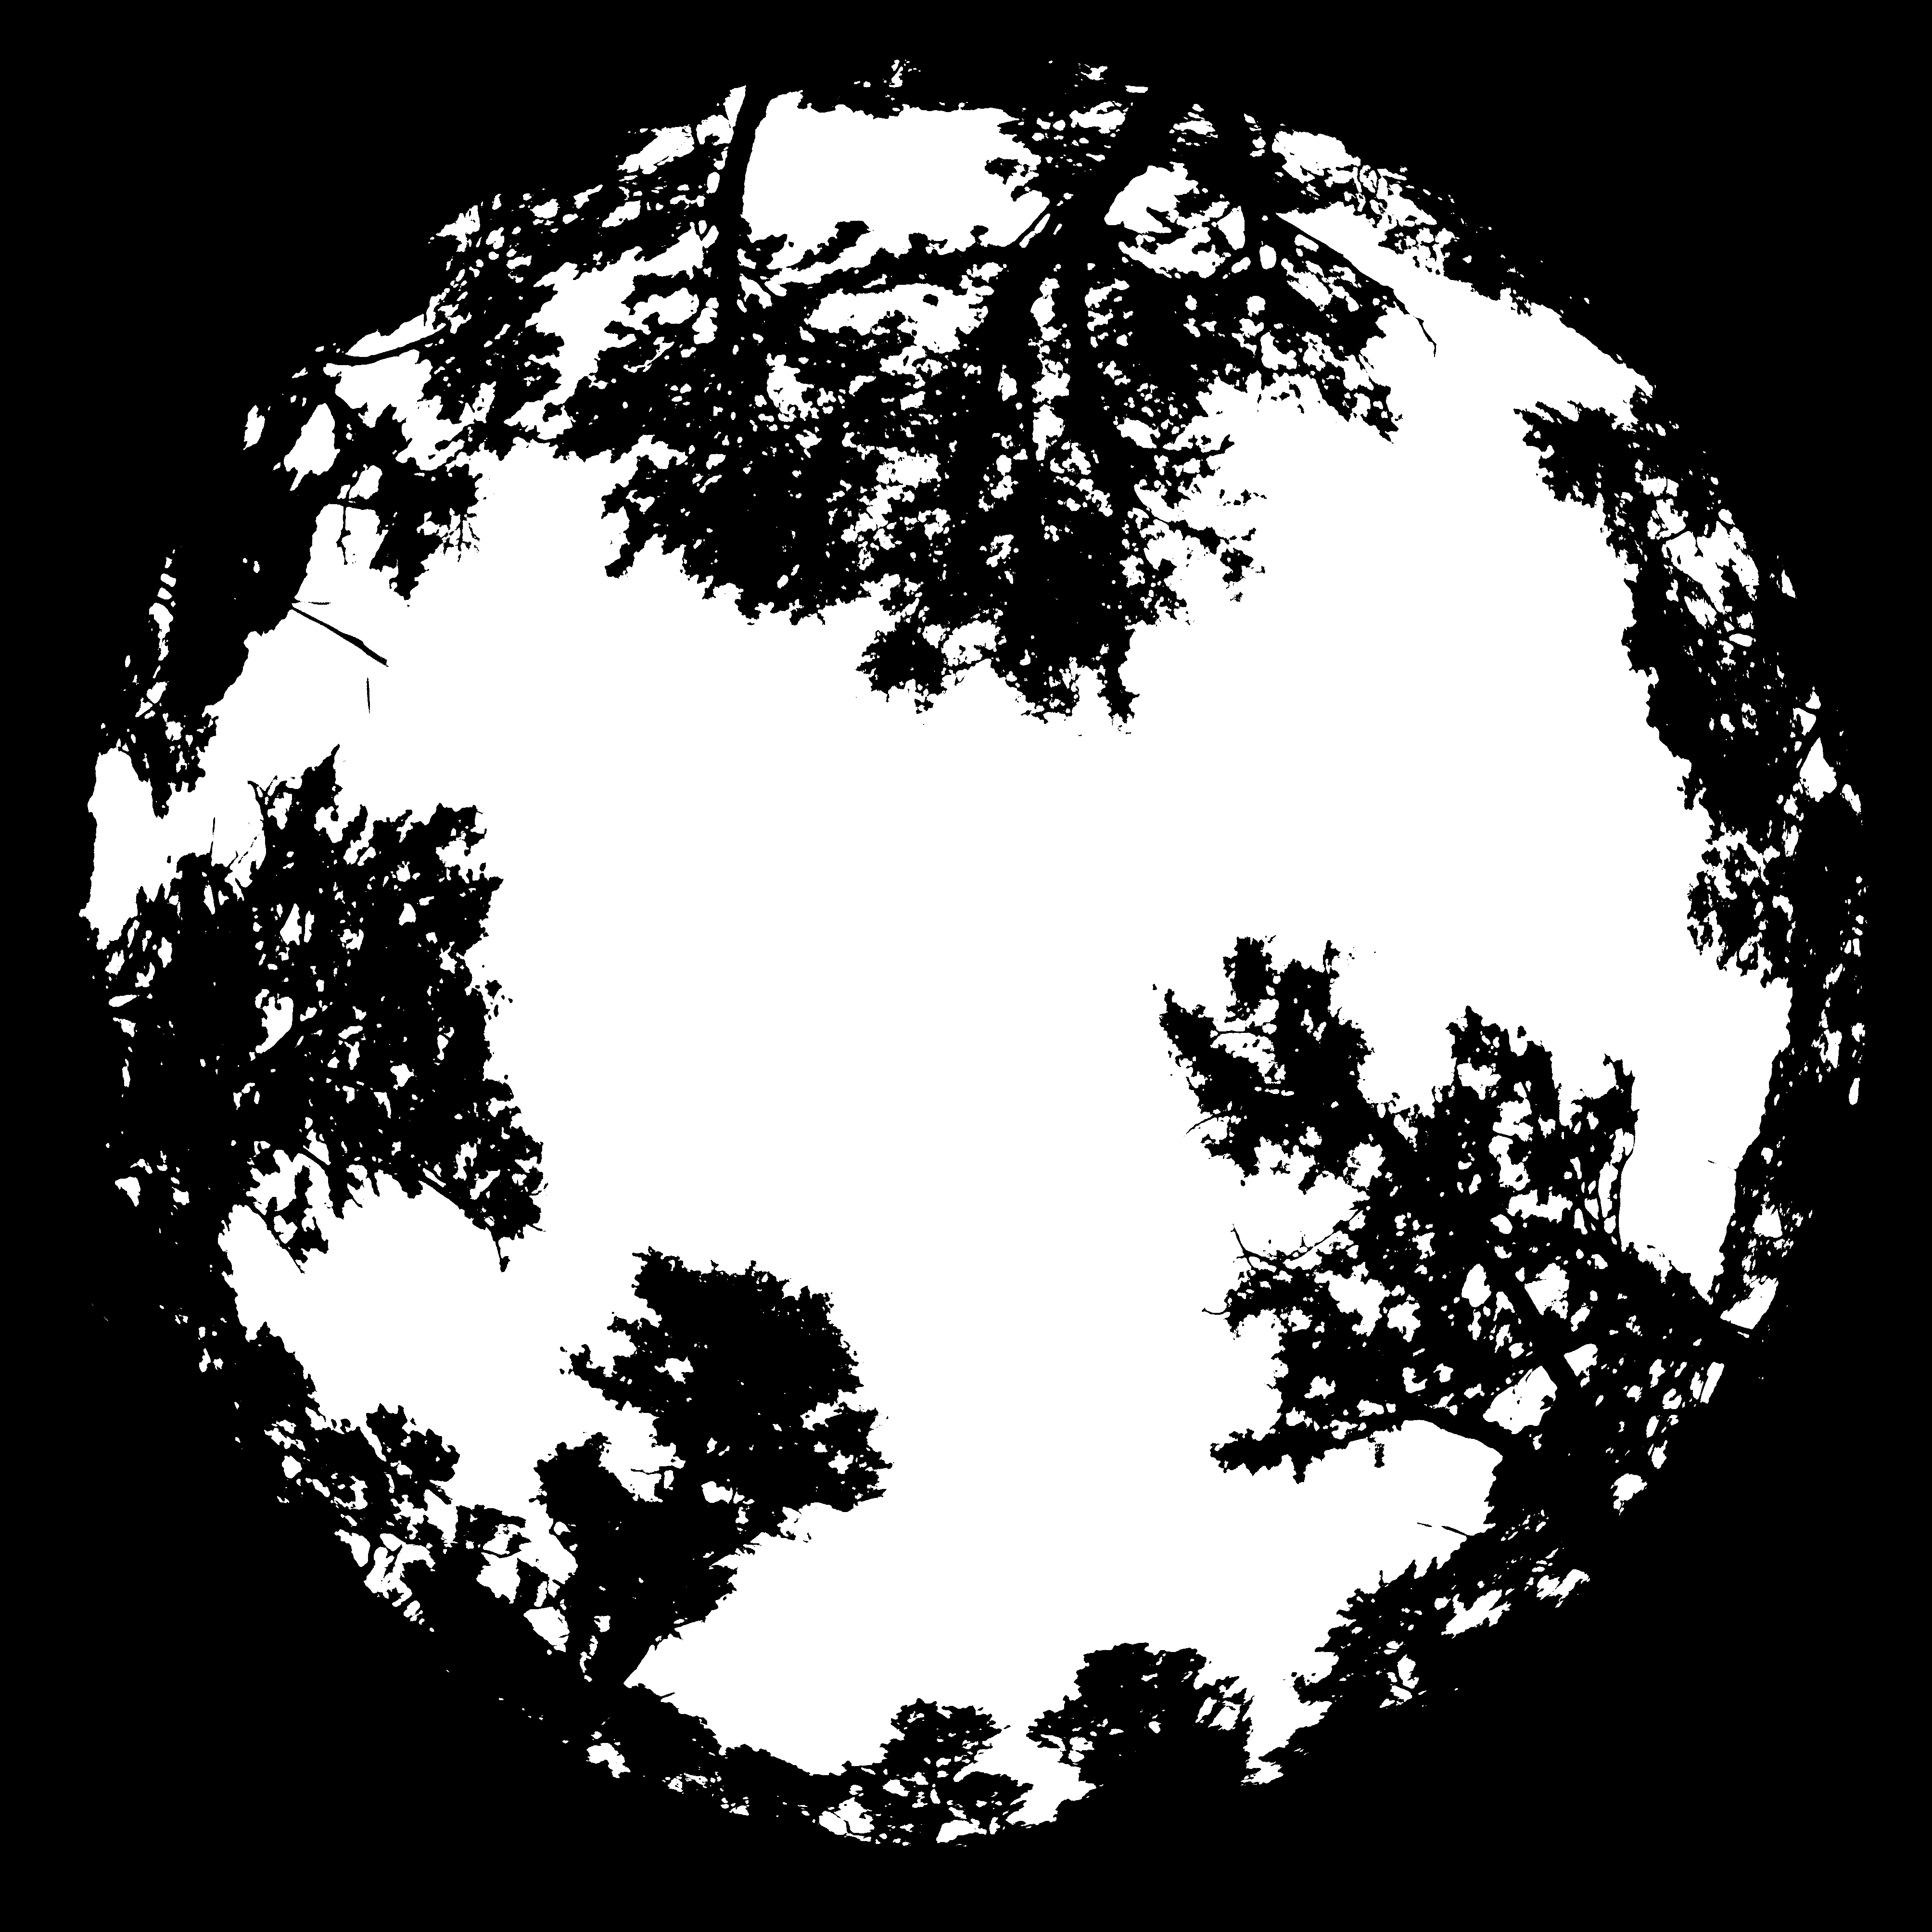
\includegraphics[width=\linewidth]{hemi_hemi}
		\caption{}
		\label{hemi_hemi}
	\end{subfigure}
	\hfill
	\begin{subfigure}{0.45\linewidth}
		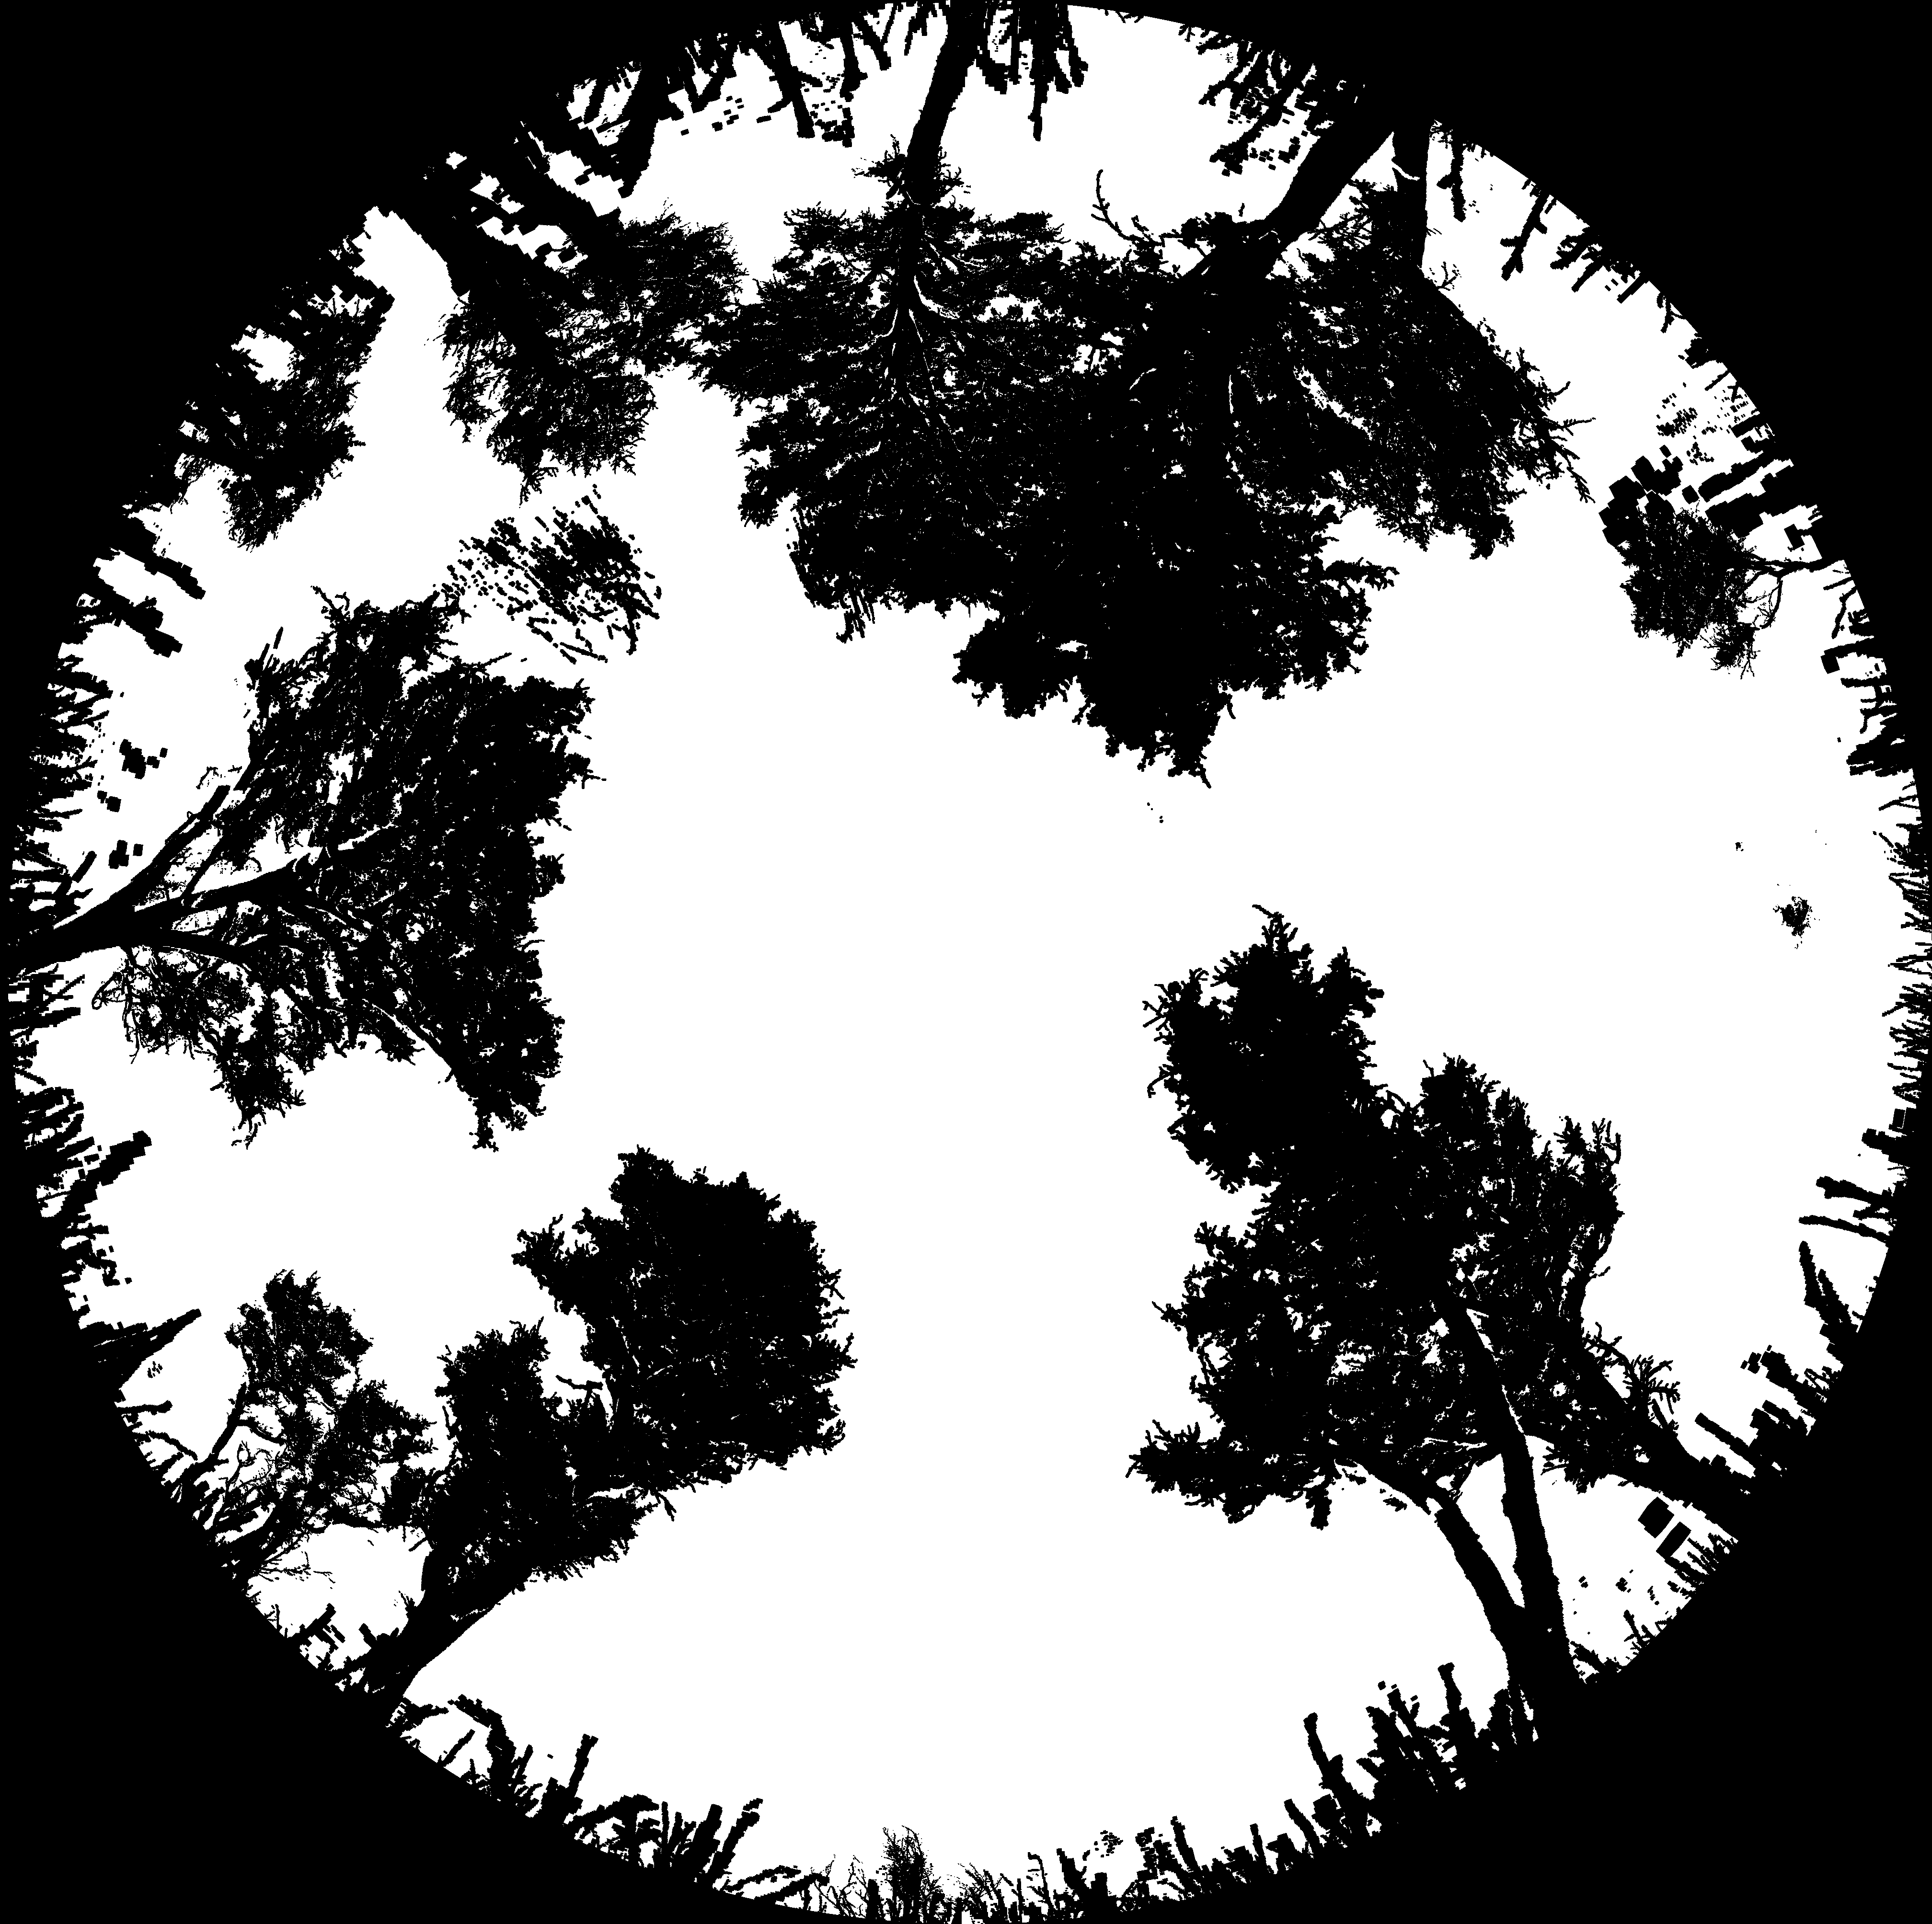
\includegraphics[width=\linewidth]{hemi_tls}
		\caption{}
		\label{hemi_tls}
	\end{subfigure}
	\caption{Comparison of hemispherical images for a subplot in Bicuar National Park, Angola. (a) A hemispherical photograph, and (b) a multi-scan point cloud modelled as cubic voxels with POV-Ray. The hemispherical photograph (left) shows some blooming, especially in the tree on the bottom right of the image, where light is seen `bleeding' through the darker canopy material, causing an under-estimation in canopy closure.}
	\label{hemi_tls_ex}
\end{figure}

\subsection{Whole plot canopy metrics}

The canopy height of each 1 ha plot was estimated using unified point clouds from all subplots. The unified point cloud was voxelised to 10 cm\textsuperscript{3}, and the 99th percentile of height from each 10 cm\textsuperscript{2} column was taken as the canopy height. Maximum height was not used as this occasionally constituted a severe outlier which skewed further 
canopy surface model smoothing. The point cloud was then cropped to the plot boundaries, located using PPK GNSS similar to the TLS targets. A pit-filling algorithm described in \citet{Khosravipour2014} was used to smooth the canopy surface model, at a resolution of 50 cm, by removing gaps within trees caused by incomplete penetration of the LiDAR beam (\autoref{P1_both}). 

\begin{figure}
	\begin{subfigure}{0.45\linewidth}
		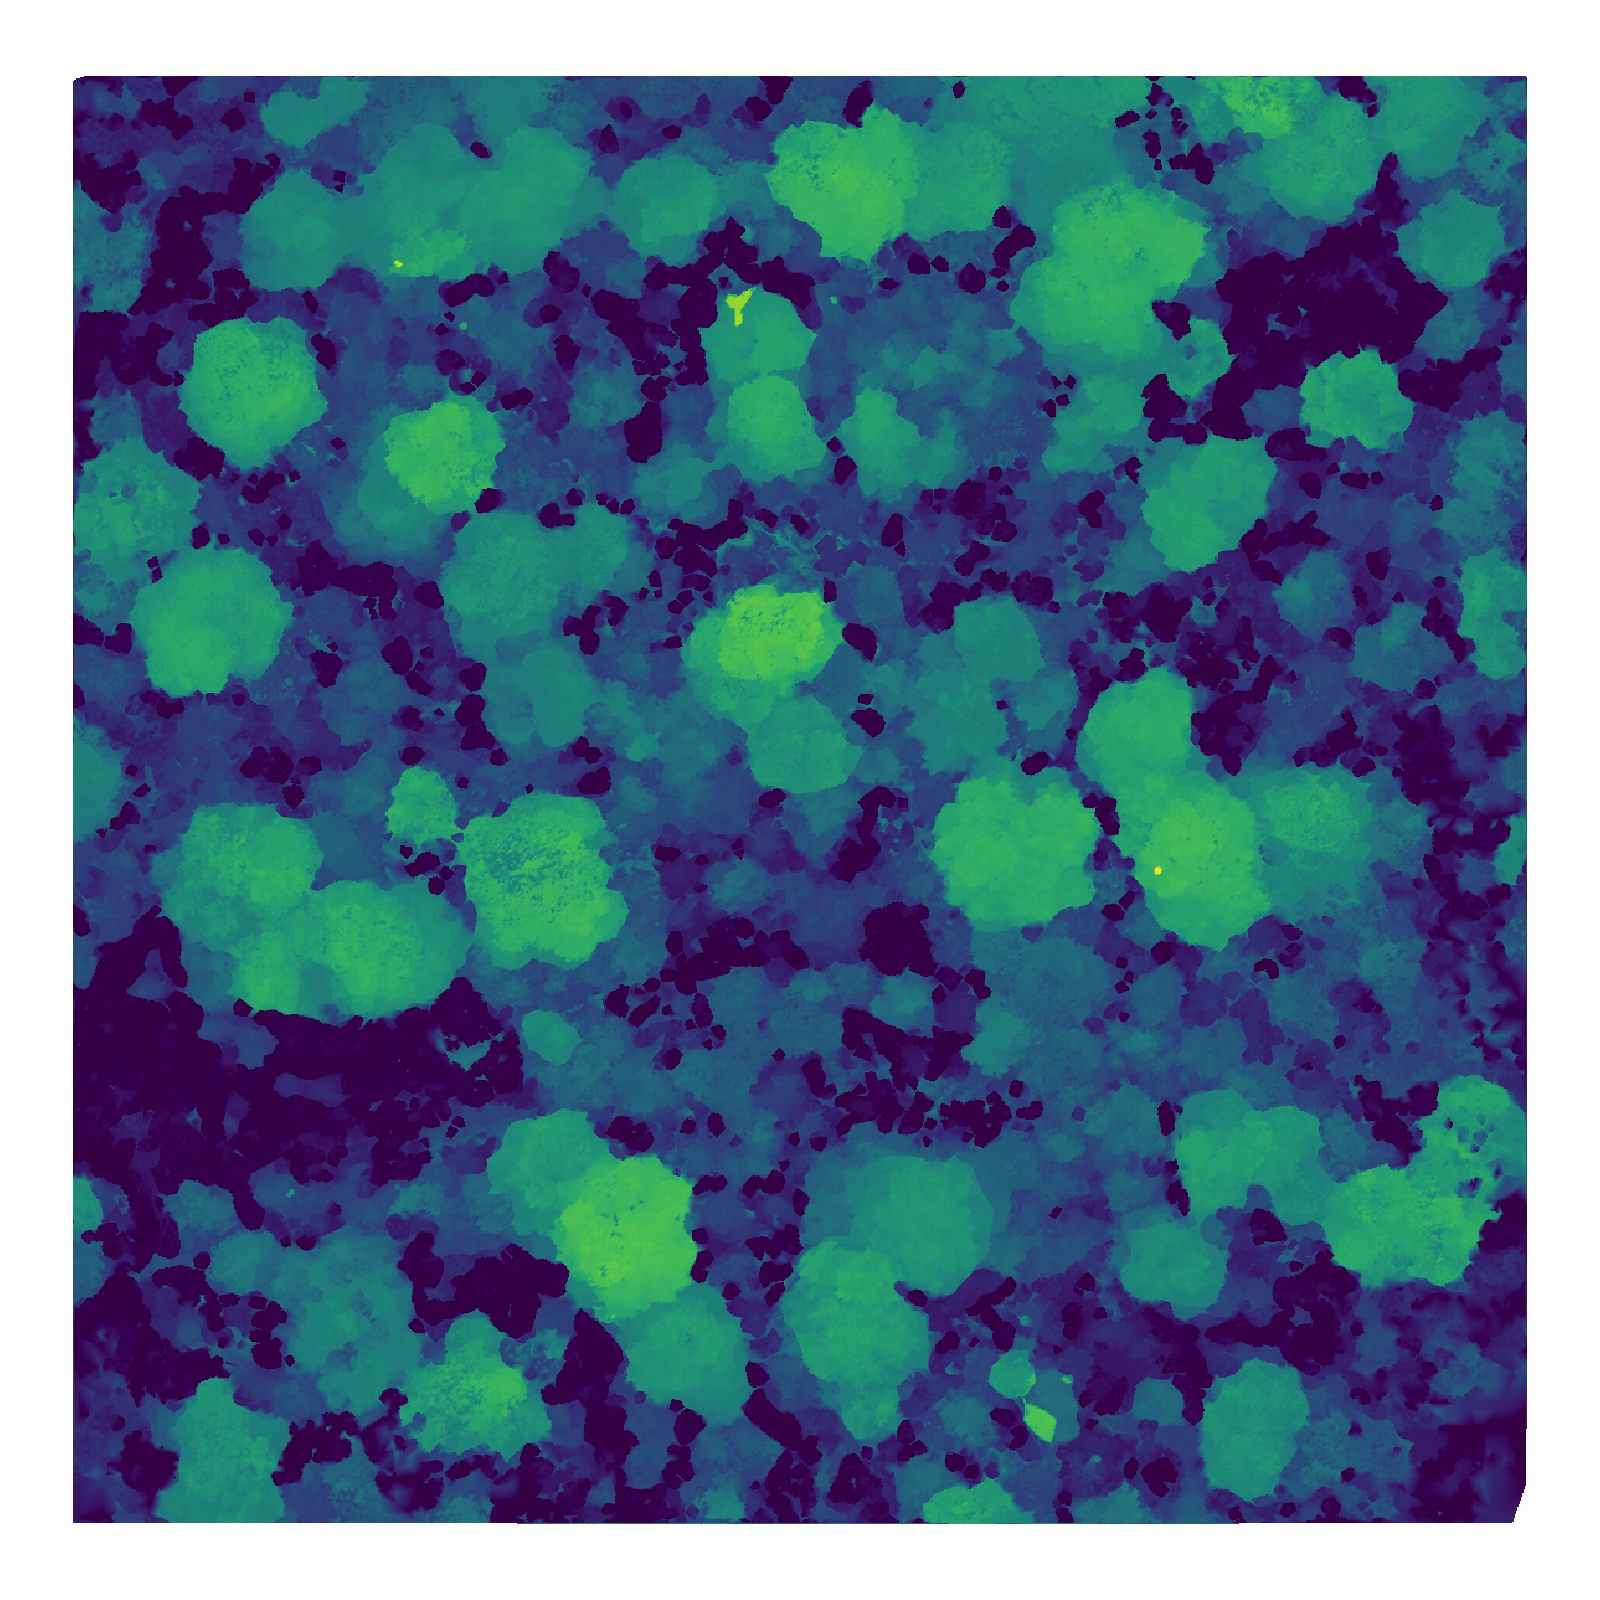
\includegraphics[width=\linewidth]{P1_raw}
		\caption{}
		\label{P1_raw}
	\end{subfigure}
	\hfill
	\begin{subfigure}{0.45\linewidth}
		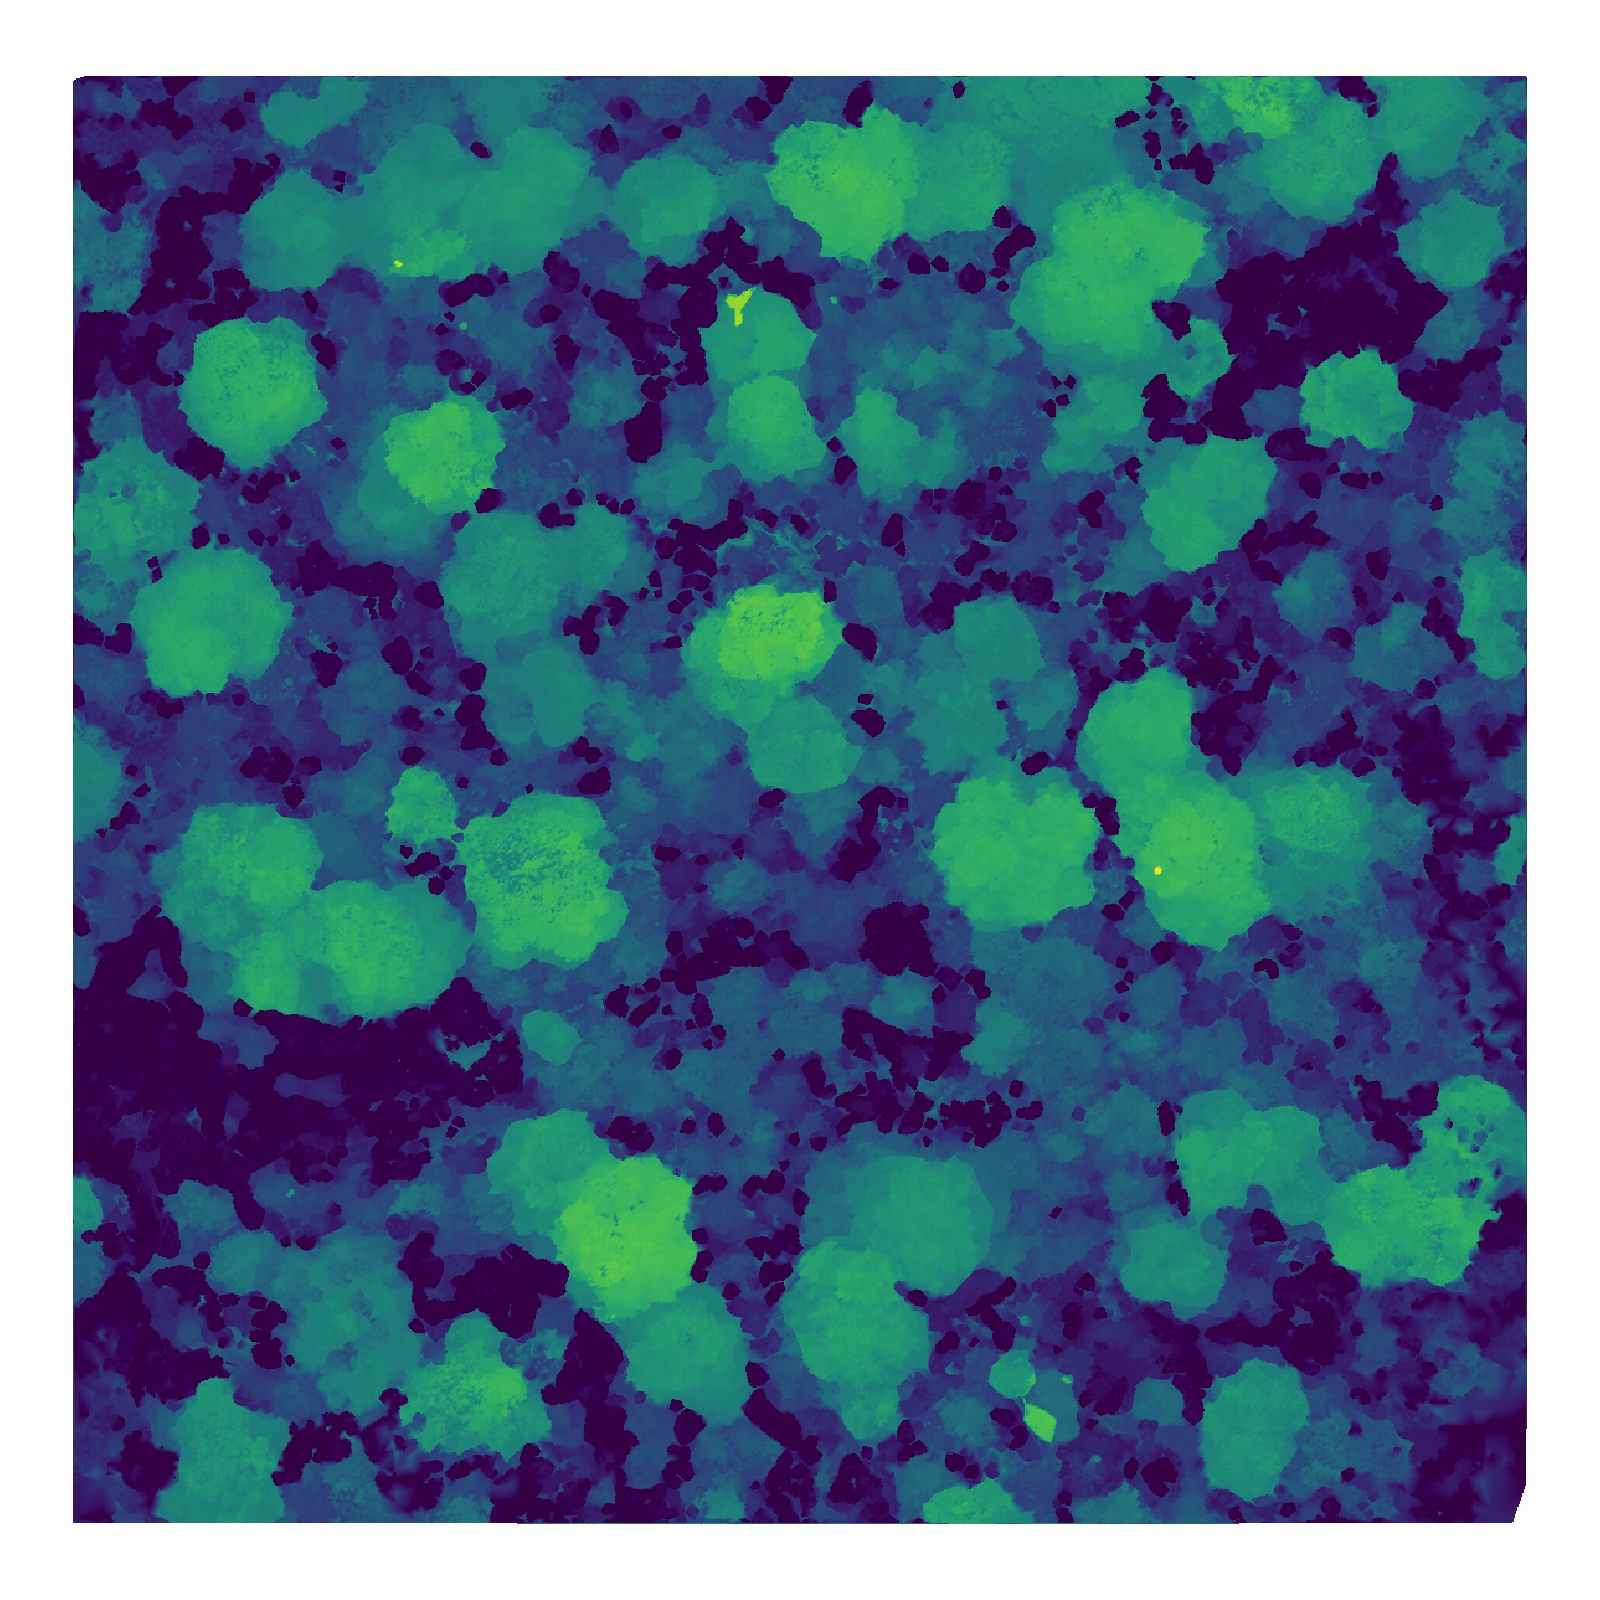
\includegraphics[width=\linewidth]{P1_pit}
		\caption{}
		\label{P1_pit}
	\end{subfigure}
	\caption{Top-down view of a 1 ha plot in Bicuar National Park. (a) The point cloud after voxelisation, noise reduction, and taking the 99th percentile of stem height in each 5 cm vertical bin. (b) The same point cloud after pit filling to generate a smooth canopy height profile. Points are coloured according to point height from the ground.}
	\label{P1_both}
\end{figure}

Mean canopy height across the plot and the coefficient of variation of canopy height were extracted from the canopy surface model for use in statistical analyses. The coefficient of variation of canopy height describes canopy structural diversity measured by the heterogeneity of the canopy surface. Other studies in closed canopy temperate and boreal forests have used metrics similar to the Topographic Roughness Index to measure canopy surface heterogeneity, by comparing canopy height to that of neighbouring pixels in the canopy height model \citep{Weligepolage2012,HerreroHuerta2020}. In this study however, the sparse nature of the tree canopies meant that these metrics were overly influenced by canopy density and the edges of individual tree canopies. Canopy rugosity ($R_{c}$) was also calculated to describe structural complexity across the entire canopy profile, rather than just the canopy surface, sensu \citet{Hardiman2011}. $R_{c}$ first calculates the standard deviation of foliage density in 50 cm\textsuperscript{2} columns across the plot ($\sigma{}G_{z}$), then calculates the standard deviation of those standard deviations: 

\begin{equation}
	R_{c} = \sigma{}(\sigma{}G_{z})_{x}
\end{equation}

Where $G_{z}$ is the vertical height axis $z$, $x$ is the horizontal axis, and $\sigma{}$ is the standard deviation. Finally, plot-level canopy closure was calculated as the mean of subplot TLS canopy closure estimates. 

\section{Stand structure metrics}

\subsection{Spatial mingling of species}

The spatial mingling index ($M_{i}$) is a spatially explicit estimate of the degree to which species are spatially mixed within a plot. Here, $M$ was calculated at the plot level as the mean of $M_{i}$ according to \citet{Gadow2002}, with the adjustment for potential neighbourhood species pool suggested by \citet{Hui2011}: 

\begin{align}
\begin{split}
	M &= \overline{M_{i}} \\
	M_{i} &= \frac{S_{i}}{n_{\text{max}}} \frac{1}{k} \sum_{j=1}^{k} v_{j} \\
	\text{with}\ v_{j} &= \begin{cases}
		0,& \text{neighbour $j$ same species as reference $i$} \\
		1,& \text{otherwise}
	\end{cases} \\
\end{split}
\end{align}

Where $k$ is the number of nearest neighbours considered for each reference tree, $S_{i}$ is the number of species found among the $k$ nearest neighbours of tree $i$, $n_{\text{max}}$ is the potential number of species in the neighbourhood, i.e. $k + 1$, and $N$ is the total number of trees in the plot. The conventional value of $k = 4$ was used here \citep{Gadow2002, Hui2004, Hui2007}. The value of $M_{i}$ increases with greater mixing of species, and all else being equal will increase with number of species within the plot (\autoref{mingling_both}).

\begin{figure}
	\begin{subfigure}{0.45\linewidth}
		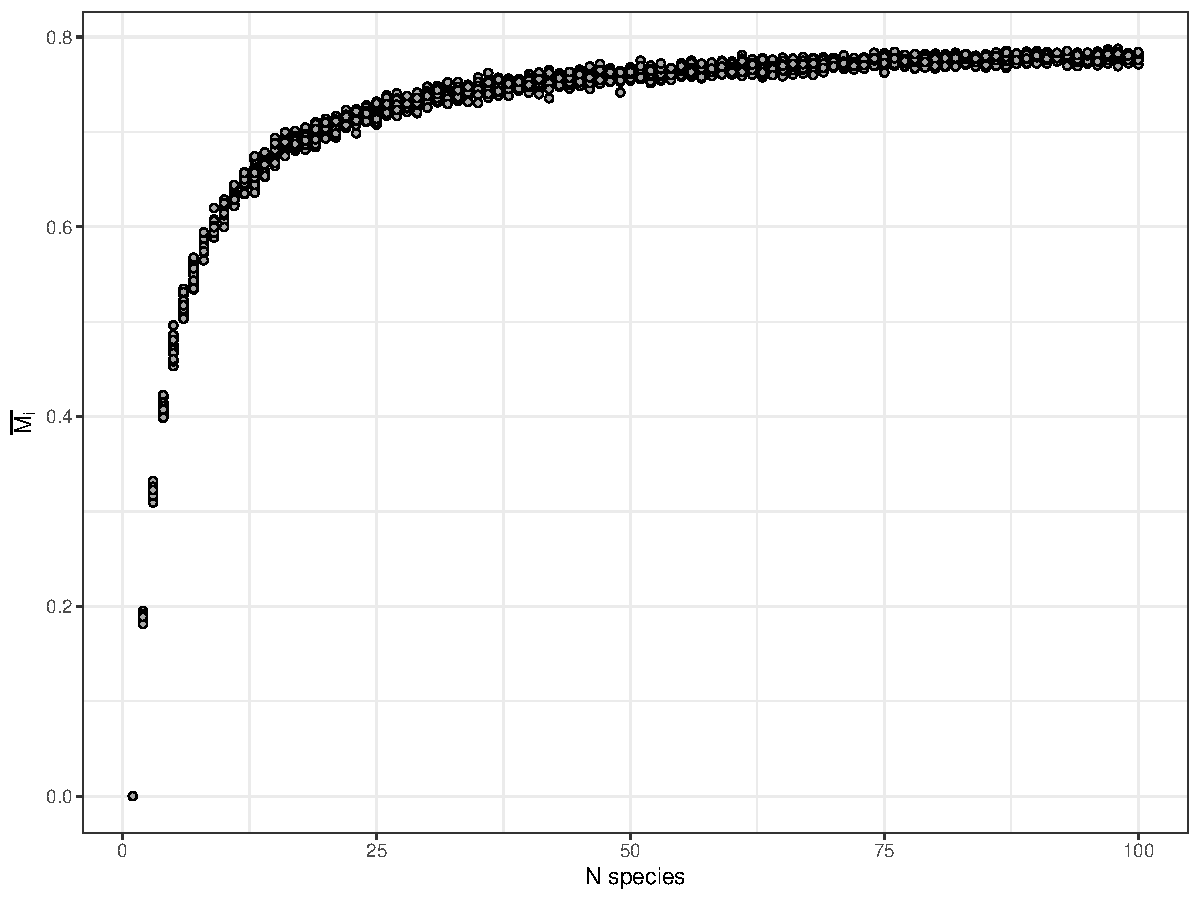
\includegraphics[width=\linewidth]{mingling_nspecies}
		\caption{}
		\label{mingling_nspecies}
	\end{subfigure}
	\hfill
	\begin{subfigure}{0.45\linewidth}
		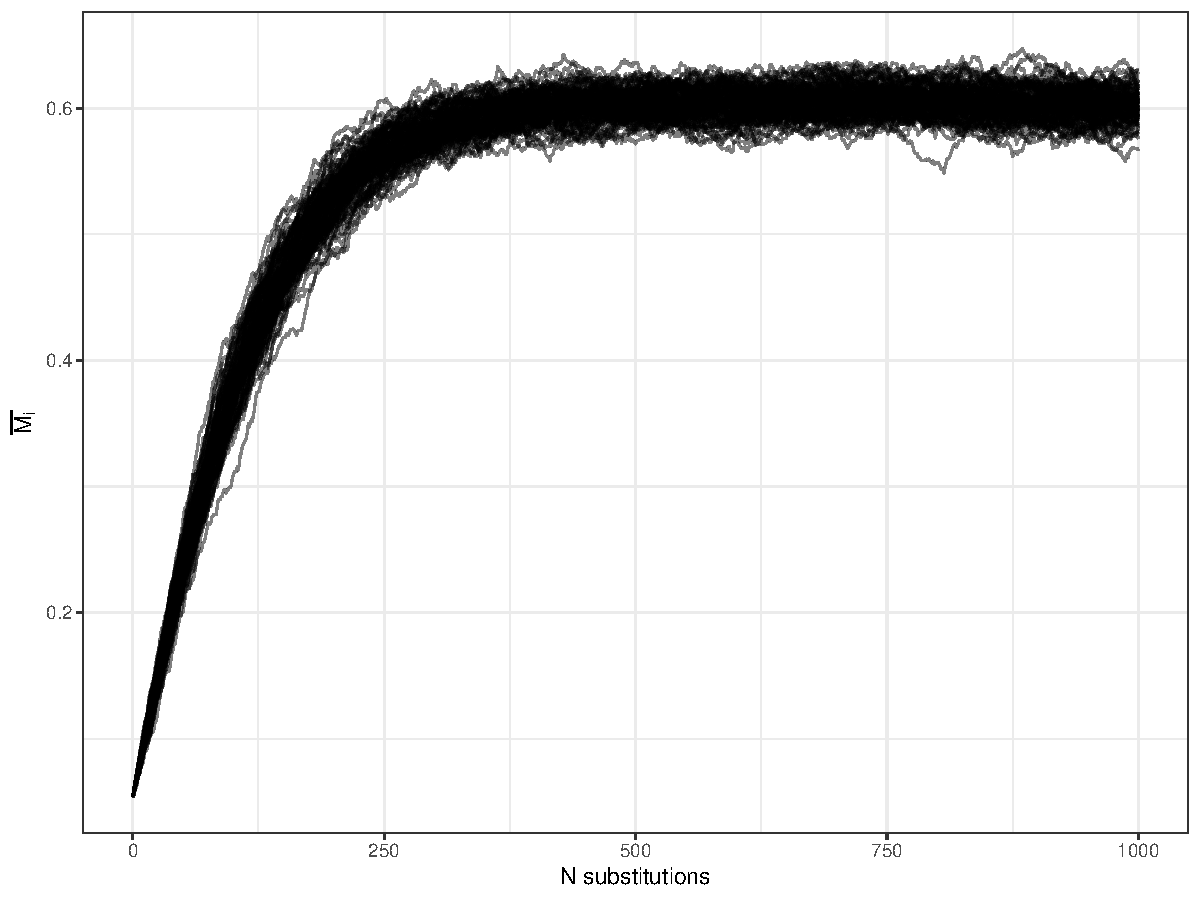
\includegraphics[width=\linewidth]{mingling_nmingl}
		\caption{}
		\label{mingling_nmingl}
	\end{subfigure}
	\caption{The behaviour of $M_{i}$ with increasing number of species (a), and increasing spatial mixing of species (b). The left panel was generated by randomly assigning different numbers of species, in equal proportions, to an evenly spaced grid of individuals. \mispreps{} replicates were conducted for each number of species. The right panel was generated by randomly swapping pairs of individuals in a plot with \minsp{} species arranged in mono-specific square blocks in an evenly spaced grid. Each line shows a single replicate, where individuals were swapped in an additive fashion, with \minreps{} total.} 
	\label{mingling_both}
\end{figure}

\subsection{Spatial clustering of stems}

The winkelmass ($W$) was calculated to estimate the degree of spatial uniformity in stem spatial distribution. Here, $W$ was calculated at the plot level as the mean of $W_{i}$) according to \citet{Gadow2002}: 

\begin{align}
\begin{split}
	W &= \overline{W_{i}} \\
	W_{i} &= \frac{1}{k} \sum_{j=1}^{k} v_{j} \\
	\text{with}\ v_{j} &= \begin{cases}
		0,& \alpha_{j} \le \alpha_{0} \\
		1,& \text{otherwise}
	\end{cases} \\
\end{split}
\end{align}

Where $k$ is the number of neighbours considered, here using the conventional value of $k = 4$, $\alpha_{j}$ is the angle between consecutive neighbours and $\alpha_{0}$ is the critical angle, where $\alpha_{0} = 360 / k$. \autoref{winkelmass} demonstrates how the value of $W_{i}$ varies according to spatial distribution of neighbours. The value of the winkelmass increases with increasing spatial clumping (decreasing spatial regularity) of individuals (\autoref{wi_diagram}), and in a plot with random tree distribution will increase as more neighbours are considered (\autoref{wi_k}).

\begin{figure}
\centering
	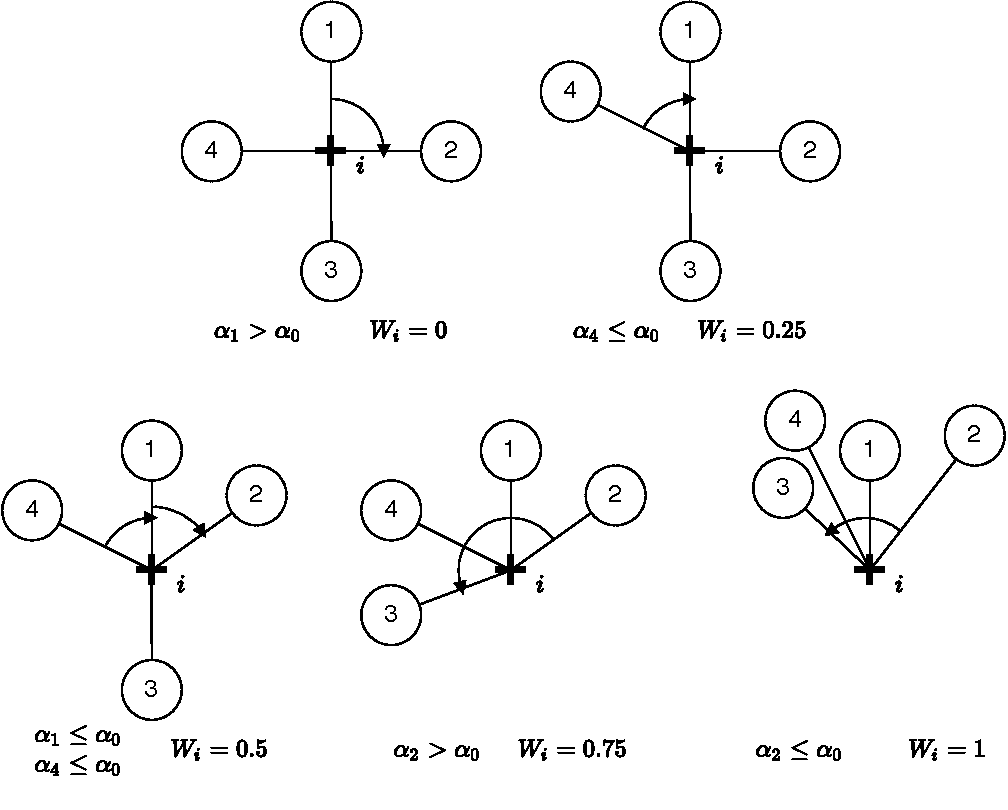
\includegraphics[width=\linewidth]{winkelmass}
	\caption{Possible values of $W_{i}$ at a sample point $i$, denoted by a cross. Neighbours are represented as circles numbered sequentially from 1 to 4, where $k = 4$. The angles of arrows in each example are given below, along with the winkelmass for that example.}
	\label{winkelmass}
\end{figure}

\begin{figure}
\centering
	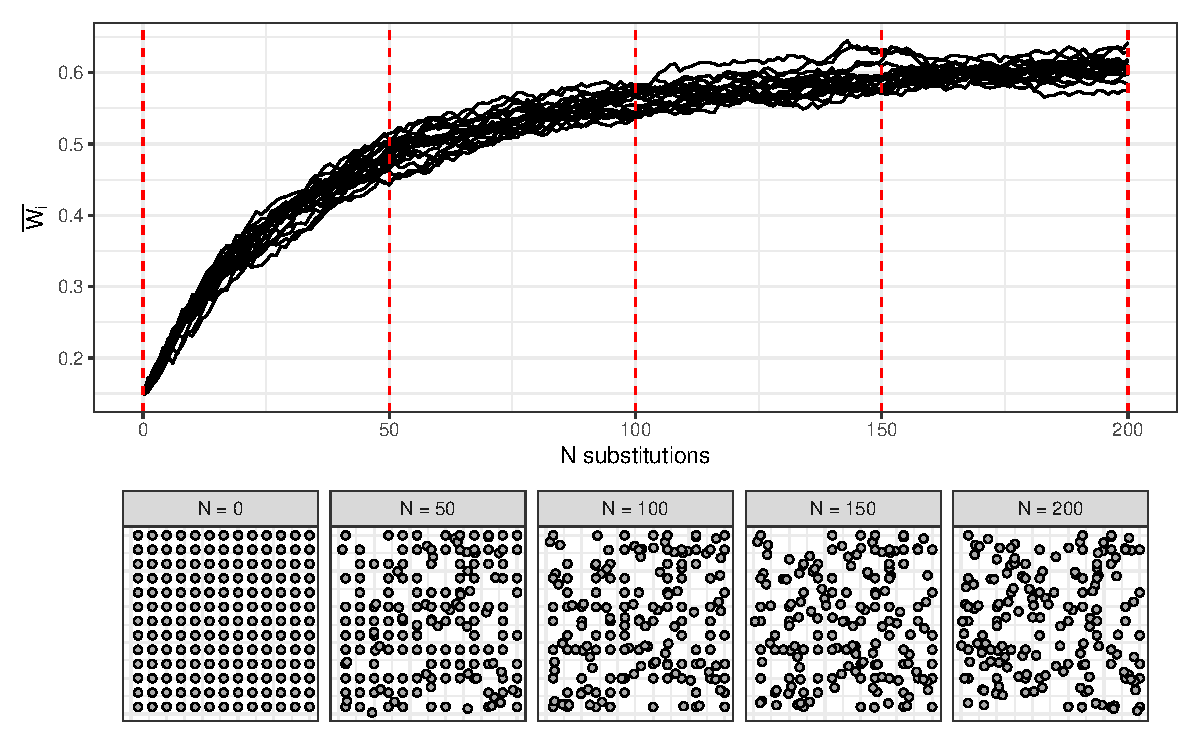
\includegraphics[width=\linewidth]{wi_diagram}
	\caption{Variation in winkelmass with increasing spatial irregularity of individuals. The top panel shows variation of winkelmass in \wireps{} plots as individuals are sequentially moved to a random location within the plot. Red dotted lines correspond to the panels below which show the spatial distribution of individuals after a given number of random individual movements.}
	\label{wi_diagram}
\end{figure}

\begin{figure}
\centering
	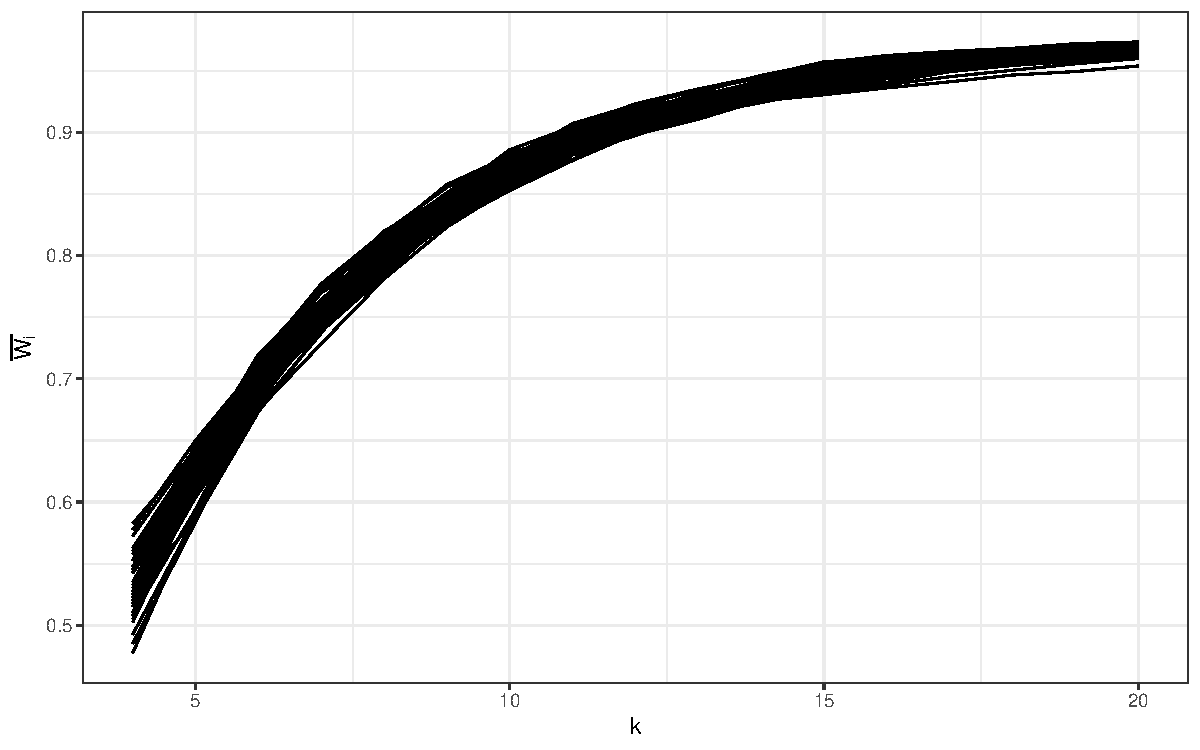
\includegraphics[width=\linewidth]{wi_k}
	\caption{Variation in winkelmass with increasing number of neighbours $k$ considered in the calculation. \wikn{} replicate plots were used, each with \wiki{} individuals randomly distributed in space.}
	\label{wi_k}
\end{figure}

\subsection{Subplot canopy crowding}

An adapted version of the Iterative Hegyi Index ($H_{i}$) was used to estimate tree spatial structure in subplots \citep{Hegyi1974}. The adapted formula used here allows the index to be based on a point rather than a focal tree, transforming it from a tree-centric competition index to a point-centric crowding index:

\begin{equation}
	H_{i} = log\sum_{j=1}^{n} (\frac{1}{L_{ij}} D_{j})
\end{equation}

Where $n$ is the number of stems with canopy material within the subplot, $D_{j}$ is the stem diameter of stem $j$ and $L_{ij}$ is the distance of stem $j$ from the subplot centre $i$. $H_{i}$ uses an iterative method for choosing active canopy occupants at the subplot centre, where the nearest individual to the subplot centre from each of 12 equally sized sectors is classified as the active stem (\autoref{hegyi}). $H_{i}$ was preferred over stem density to describe stem crowding in subplots because it is sensitive to how close a stem is to the subplot centre, which will affect canopy closure even if the number of stems in the subplot remains the same. 

\begin{figure}
	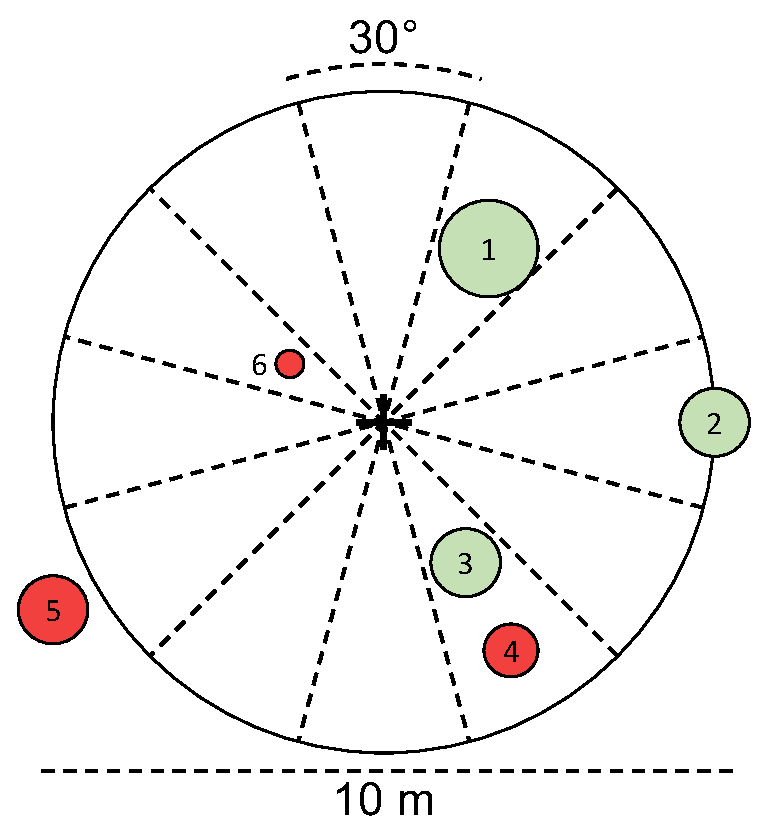
\includegraphics[width=0.6\linewidth]{hegyi}
	\caption{Schematic diagram demonstrating use of the Iterative Hegyi Index to assess crowding within each subplot. The 10 metre diameter subplot is divided into 12 equally sized sectors. Within each sector, the nearest stem of sufficient size (>5 cm diameter) to the subplot centre is recorded (e.g. 1). All stems with any canopy material inside the subplot are valid (e.g. 2). Stem 4 is not valid as it is behind stem 3. Stem 5 is invalid as all its canopy is outside the subplot. Stem 6 is too small to be recorded.}
	\label{hegyi}
\end{figure}

\FloatBarrier{}
\printbibliography

\end{document}

